% ============================================================================
%  PLANTILLA MONOGRÁFICA DE ALTO RENDIMIENTO — ACADÉMICA Y FÍSICA
%  TRABAJO DE INVESTIGACIÓN FORMATIVA (TIF) — FASE II
%  CURSO: FÍSICA I
%  ESCUELA PROFESIONAL DE INGENIERÍA PESQUERA — UNSA
% ============================================================================

\documentclass[11pt,a4paper]{article}

% ─── Paquetes de Idioma y Codificación ──────────────────────────────────────
\usepackage[utf8]{inputenc}
\usepackage[T1]{fontenc}
\usepackage[spanish,es-tabla]{babel}

% ─── Tipografía y Diseño de Fuentes Premium ─────────────────────────────────
\usepackage{charter} % Fuente Serif Charter (altamente legible y elegante)
% removed mathdesign to avoid font and symbol conflicts % Complemento matemático elegante
\usepackage[scaled=0.92]{helvet} % Sans-serif para encabezados y detalles
\renewcommand{\familydefault}{\rmdefault}
\usepackage{type1cm} % Permite escalado libre de fuentes para evitar advertencias de tamaño 5.5pt


% ─── Geometría y Márgenes (Formato APA / Journal Híbrido) ───────────────────
\usepackage[
    a4paper,
    top=2.54cm,
    bottom=2.54cm,
    left=2.54cm,
    right=2.54cm,
    headheight=20pt,
    headsep=15pt,
    footskip=30pt
]{geometry}
\usepackage{setspace}
\onehalfspacing

% ─── Colores Estilo "Oceanic Science" (Evolución de la plantilla clásica) ──
\usepackage[dvipsnames,svgnames]{xcolor}
\definecolor{oceanPrimary}{HTML}{0B2545}   % Azul marino profundo (Títulos)
\definecolor{oceanSecondary}{HTML}{134074} % Azul medio (Subtítulos)
\definecolor{oceanAccent}{HTML}{00B4D8}    % Turquesa/Cian (Acentos y Vectores)
\definecolor{oceanDark}{HTML}{03071E}      % Gris casi negro para texto principal
\definecolor{oceanBoxBg}{HTML}{F4F7F6}     % Fondo cálido de cajas de texto
\definecolor{vectorGreen}{HTML}{10B981}    % Verde para fuerza de sostentación del casco
\definecolor{vectorRed}{HTML}{EF4444}      % Rojo para peso

% ─── Paquetes Matemáticos y Físicos de Alta Precisión ──────────────────────
\usepackage{amsmath}
\usepackage{amsfonts}
\usepackage{amssymb}
\usepackage{bm} % Vectores en negrita cursiva
\usepackage{siunitx} % Unidades del SI estandarizadas
\sisetup{locale=FR, per-mode=symbol}

% ─── Gráficos, TikZ y Diagramas Vectoriales ─────────────────────────────────
\usepackage{graphicx}
\usepackage{float}
\usepackage{booktabs}
\usepackage{tabularx}
\usepackage{multirow}
\usepackage{tikz}
\usetikzlibrary{shapes.geometric, arrows.meta, positioning, calc, patterns, babel}

% ─── Fondo de Marca de Agua sutil para Autores ──────────────────────────────
\usepackage{eso-pic}
\AddToShipoutPictureFG{%
    \ifnum\value{page}>1
        \AtPageCenter{%
            \begin{tikzpicture}[remember picture, overlay]
                % Faded grayscale watermark logos in the background (UNSA and Fisheries School)
                % Placed diagonally at (-6,-6) and (6,6) and rotated 45 degrees to match the text orientation
                \node[opacity=0.15, rotate=45] at (-6,-6) {
\includegraphics[width=5.0cm]{logo_unsa_watermark.png}};
                \node[opacity=0.15, rotate=45] at (6,6) {
\includegraphics[width=5.0cm]{logo_pesquera_watermark.png}};
                
                % Rotated author names stacked in a robust tabular environment (using neutral gray for watermark consistency)
                \node[rotate=45, text=black!65, text opacity=0.30] at (0,0) {%
                    \begin{tabular}{c}
                        \fontsize{14pt}{17pt}\selectfont\sffamily\bfseries ING. FRANCO ARENAS \\[6pt]
                        \fontsize{12pt}{15pt}\selectfont\sffamily\bfseries EST. ELISVAN CHUMBISLLA \\[6pt]
                        \fontsize{12pt}{15pt}\selectfont\sffamily\bfseries EST. JHON APUCUSI \\[6pt]
                        \fontsize{12pt}{15pt}\selectfont\sffamily\bfseries EST. KAIT LUPO
                    \end{tabular}
                };
            \end{tikzpicture}
        }%
    \fi
}

% ─── Encabezado y Pie de Página Customizados (Estilo Libro Académico) ───────
\usepackage{fancyhdr}
\usepackage{lastpage}
\pagestyle{fancy}
\fancyhf{}

% Encabezados limpios (sin logotipos repetitivos en cada hoja)
\lhead{\fontsize{9pt}{11pt}\selectfont\sffamily\color{oceanSecondary} TIF: Análisis Físico del Sistema de Izaje Pesquero}
\rhead{\fontsize{9pt}{11pt}\selectfont\sffamily\color{oceanSecondary} E.P. Ingeniería Pesquera --- UNSA}

% Pies de página
\lfoot{\fontsize{9pt}{11pt}\selectfont\sffamily\color{oceanSecondary} Arequipa, 2026}
\rfoot{\fontsize{9pt}{11pt}\selectfont\sffamily\color{oceanSecondary} Página \thepage\ de \pageref{LastPage}}

\renewcommand{\headrulewidth}{1.5pt}
\renewcommand{\footrulewidth}{0.6pt}
\renewcommand{\headrule}{%
    {\color{oceanPrimary}\hrule width\headwidth height\headrulewidth \vskip-\headrulewidth}%
}
\renewcommand{\footrule}{%
    {\color{oceanSecondary}\vskip-\footruleskip\vskip-\footrulewidth
    \hrule width\headwidth height\footrulewidth\vskip\footruleskip}%
}

% ─── Títulos de Sección (Norma APA 7ma Edición) ─────────────────────────────
\usepackage{titlesec}
\titleformat{\section}
    {\fontsize{12pt}{14pt}\selectfont\sffamily\bfseries\color{oceanPrimary}\centering}
    {\thesection.}
    {0.5em}
    {}

\titleformat{\subsection}
    {\fontsize{11pt}{13pt}\selectfont\sffamily\bfseries\color{oceanSecondary}}
    {\thesubsection.}
    {0.5em}
    {}

\titleformat{\subsubsection}
    {\fontsize{10.5pt}{12.5pt}\selectfont\sffamily\bfseries\itshape\color{oceanSecondary!80!black}}
    {\thesubsubsection.}
    {0.5em}
    {}

\titlespacing*{\section}{0pt}{18pt}{8pt}
\titlespacing*{\subsection}{0pt}{14pt}{6pt}
\titlespacing*{\subsubsection}{0pt}{12pt}{4pt}

% ─── Tabla de Contenidos Estilizada ─────────────────────────────────────────
\usepackage{tocloft}
\renewcommand{\cftsecfont}{\sffamily\bfseries\color{oceanPrimary}}
\renewcommand{\cftsecpagefont}{\sffamily\bfseries\color{oceanPrimary}}
\renewcommand{\cftsubsecfont}{\sffamily\color{oceanSecondary}}
\renewcommand{\cftsubsecpagefont}{\sffamily\color{oceanSecondary}}
\renewcommand{\cftsecleader}{\cftdotfill{\cftdotsep}}

% ─── Hiperenlaces y Metadatos PDF ───────────────────────────────────────────
\usepackage[
    colorlinks=true,
    linkcolor=oceanSecondary,
    citecolor=Maroon,
    urlcolor=oceanAccent!80!black,
    bookmarks=true,
    bookmarksnumbered=true,
    pdfauthor={Arenas Mamani, Chumbislla Sullca, Apucusi Mamani, Lupo Ziabala},
    pdftitle={Análisis físico del sistema de izaje en embarcaciones de cerco: Relación entre Tensión, Torque y Potencia durante la extracción de captura},
    pdfsubject={Trabajo de Investigación Formativa (TIF) --- Física I},
    pdfkeywords={Tensión, Torque, Potencia, Corriente Marina, Dinámica, Bonito, UNSA}
]{hyperref}

% ─── Personalización de Listas ──────────────────────────────────────────────
\usepackage{enumitem}
\setlist[itemize]{leftmargin=1.0cm, itemsep=3pt, parsep=1pt}
\setlist[enumerate]{leftmargin=1.0cm, itemsep=3pt, parsep=1pt}

% ─── Leyendas (Captions) de Figuras y Tablas ────────────────────────────────
\usepackage[
    font={small,color=oceanDark},
    labelfont={sf,bf,color=oceanPrimary},
    labelsep=period,
    justification=centering,
    singlelinecheck=false
]{caption}

% ─── Cajas de Texto y Notas Especiales (tcolorbox) ─────────────────────────
\usepackage{tcolorbox}
\tcbuselibrary{skins,breakable}

\newtcolorbox{physbox}[1][]{%
    colback=oceanBoxBg,
    colframe=oceanPrimary,
    coltitle=white,
    fonttitle=\sffamily\bfseries\small,
    boxrule=1pt,
    arc=4pt,
    left=10pt,right=10pt,top=8pt,bottom=8pt,
    breakable,
    shadow={2pt}{-2pt}{0pt}{black!10},
    #1
}

% ============================================================================
%                         INICIO DEL DOCUMENTO
% ============================================================================
\begin{document}

% ──────────────────────────────────────────────────────────────────────────
%  PORTADA ACADÉMICA FORMAL (MONOGRAFÍA/JOURNAL HÍBRIDO)
% ──────────────────────────────────────────────────────────────────────────
\begin{titlepage}
    \begin{tikzpicture}[remember picture, overlay]
        % Marco decorativo de doble borde
        \draw[line width=1.5pt, color=oceanPrimary] ($(current page.north west) + (1.5cm,-1.5cm)$) rectangle ($(current page.south east) + (-1.5cm,1.5cm)$);
        \draw[line width=0.5pt, color=oceanSecondary] ($(current page.north west) + (1.65cm,-1.65cm)$) rectangle ($(current page.south east) + (-1.65cm,1.65cm)$);
    \end{tikzpicture}
    
    \centering
    \vspace*{0.5cm}
    
    {\fontsize{14pt}{16pt}\selectfont\sffamily\bfseries\color{oceanPrimary} UNIVERSIDAD NACIONAL DE SAN AGUSTÍN DE AREQUIPA} \\[\baselineskip]
    {\fontsize{11pt}{13pt}\selectfont\sffamily\color{oceanSecondary} FACULTAD DE PROCESOS} \\
    {\fontsize{11pt}{13pt}\selectfont\sffamily\color{oceanSecondary} ESCUELA PROFESIONAL DE INGENIERÍA PESQUERA} \\
    
    \vspace{1.0cm}
    \begin{minipage}{0.45\textwidth}
        \centering
        
\includegraphics[height=3.4cm]{logo_unsa_clean.png}
    \end{minipage}
    \hfill
    \begin{minipage}{0.45\textwidth}
        \centering
        
\includegraphics[height=3.4cm]{logo_pesquera_clean.png}
    \end{minipage}
    \vspace{1.0cm}
    
    {\fontsize{10pt}{12pt}\selectfont\sffamily\bfseries\color{oceanSecondary} TRABAJO DE INVESTIGACIÓN FORMATIVA (TIF) --- FASE II} \\
    \vspace{0.6cm}
    
    \begin{tcolorbox}[
        colback=oceanPrimary!5,
        colframe=oceanPrimary,
        arc=6pt,
        boxrule=1.5pt,
        center,
        width=0.9\textwidth,
        halign=center
    ]
        \fontsize{13pt}{16pt}\selectfont\sffamily\bfseries\color{oceanPrimary}
        ANÁLISIS FÍSICO DEL SISTEMA DE IZAJE EN EMBARCACIONES DE CERCO: RELACIÓN ENTRE TENSIÓN, TORQUE Y POTENCIA DURANTE LA EXTRACCIÓN DE CAPTURA
    \end{tcolorbox}
    
    \vspace{1.5cm}
    
    \begin{minipage}{0.85\textwidth}
        \fontsize{10pt}{12pt}\selectfont\sffamily
        \begin{tabular}{ll}
            \textbf{Curso:} & Física I \\
            \textbf{Docente:} & Mag. Whinders Joel Fernandez Granda \\
            \textbf{Grupo de Trabajo:} & \\
            --- Franco Alessandro Arenas Mamani & (CUI: 20191977) \\
            --- Elisvan Chumbislla Sullca & (CUI: 20260171) \\
            --- Jhon Diego Apucusi Mamani & (CUI: 20260168) \\
            --- Kait Fatima Lupo Ziabala & (CUI: 20260180) \\
        \end{tabular}
    \end{minipage}
    
    \vfill
    
    {\fontsize{10pt}{12pt}\selectfont\sffamily\color{oceanSecondary} Arequipa, Perú \\ 2026}
\end{titlepage}


\newpage
\thispagestyle{plain}
\tableofcontents
\newpage

% ──────────────────────────────────────────────────────────────────────────
%  CUERPO DEL INFORME
% ──────────────────────────────────────────────────────────────────────────

\section{Introducción y Contexto}
El sector pesquero industrial en el Perú destaca globalmente por el volumen de extracción de recursos marinos, siendo la anchoveta y las especies pelágicas de mayor tamaño, como el pez Bonito (\textit{Sarda chiliensis})\footnote{El pez Bonito es una especie pelágica transzonaria de gran importancia comercial en la costa peruana, caracterizada por una carne rica en ácidos grasos y una densidad corporal promedio de \SI{1050}{kg/m^3}.}, pilares en la cadena de Consumo Humano Directo (CHD) e Indirecto (CHI) (FAO, 2022). La operatividad eficiente a bordo de estas naves depende críticamente de los equipos de cubierta, de los cuales el sistema de izaje (winche hidráulico o mecánico y juego de poleas) es el eje central para virar la red de cerco.

Desde la perspectiva de la física clásica, el izaje de una red cargada con biomasa representa un problema de mecánica clásica. El sistema debe contrarrestar fuerzas dinámicas: el peso de la masa extraída y la fuerza hidrodinámica de arrastre provocada por el agua de mar y las corrientes marinas transversales. Comprender y modelar estos fenómenos mecánicos permite asegurar que el winche, el eje y los motores marinos auxiliares trabajen en rangos de eficiencia y seguridad operativa adecuados, previniendo fallos críticos de fatiga y ruptura del cableado (García et al., 2019).


\section{Planteamiento del Problema}

\subsection{Observación de Campo}
Durante la maniobra de recolección de captura (virado) en una embarcación de cerco, el cable principal que une el winche con la pluma de carga es sometido a tensiones dinámicas importantes. El motor que acciona el tambor del winche debe proporcionar un torque suficiente para vencer estas cargas debidas a la tracción del peso y las fuerzas hidrodinámicas de arrastre de la corriente marina. Si no se dimensiona adecuadamente la relación de torque y potencia del motor auxiliar con respecto a la biomasa capturada y la corriente, el sistema puede sobrecargarse, provocando la deformación plástica del eje de transmisión o la falla mecánica de los cables de izaje (Serway \& Jewett, 2018).

\subsection{Definición del Problema}
¿De qué manera las variables dinámicas de masa de la captura de bonito, el arrastre hidrodinámico y la inclinación del cable inducida por las corrientes marinas determinan el perfil de tensiones mecánicas en el cable principal, el torque en el tambor del winche y la potencia mínima requerida en los motores marinos auxiliares a fin de garantizar un izaje seguro y constante de \SI{500}{kg} de biomasa?

\section{Modelado Físico y Análisis Vectorial (Marco Teórico)}
Para resolver las demandas de potencia y par torsor en el diseño del winche, se establece un modelo vectorial bidimensional ($x, y$) en el plano vertical, donde el eje $y$ apunta en dirección opuesta a la gravedad.

\subsection{Caracterización Vectorial de Fuerzas}
El Diagrama de Cuerpo Libre (DCL) de la red cargada con pez bonito se compone de tres fuerzas fundamentales, las cuales gobiernan la dinámica del sistema de acuerdo con los principios de la mecánica clásica (Young \& Freedman, 2018):
\begin{enumerate}
    \item \textbf{Vector Peso ($\vec{P}$):} Actúa verticalmente hacia abajo debido a la atracción gravitatoria sobre la masa de la captura ($m$) y la estructura de la red ($m_{\text{red}}$) (Hewitt, 2016), y se expresa en la ecuación \eqref{eq:peso}:
    \begin{equation}\label{eq:peso}
    \vec{P} = -(m + m_{\text{red}}) \cdot g \hat{j}
    \end{equation}
    \item \textbf{Vector de Arrastre Hidrodinámico ($\vec{F}_d$):} Resistencia al avance viscoso de la malla y el pescado en el agua, actuando en dirección opuesta a la velocidad de la red relativa al agua $\vec{v}_{\text{rel}}$ (Young \& Freedman, 2018). Debido a la existencia de corrientes marinas transversales, este vector posee componentes tanto horizontales como verticales, actuando en un ángulo $\phi$ respecto a la vertical:
    \begin{equation}\label{eq:arrastre_vec}
    \vec{F}_d = -F_d \sin\phi \hat{i} - F_d \cos\phi \hat{j}
    \end{equation}
    Donde la magnitud $F_d$ está determinada por la velocidad relativa del flujo:
    \begin{equation}\label{eq:arrastre_mag_teorica}
    F_d = \frac{1}{2} C_d \cdot \rho_{\text{agua}} \cdot A_{\text{proy}} \cdot v_{\text{rel}}^2
    \end{equation}
    \item \textbf{Vector Tensión del Cable ($\vec{T}$):} Fuerza de tracción ejercida por el cable del winche a través del polipasto. Debido a la deriva de la embarcación y el arrastre lateral de la corriente, el cable forma un ángulo $\theta$ con respecto a la vertical:
    \begin{equation}\label{eq:tension_vec}
    \vec{T} = T \sin\theta \hat{i} + T \cos\theta \hat{j}
    \end{equation}
\end{enumerate}

\begin{figure}[H]
\centering
\caption{Diagrama de Cuerpo Libre (DCL) de la captura de Bonito con descomposición angular.}
\label{fig:dcl_tikz}
\vspace{0.2cm}
\begin{tikzpicture}[scale=1.3]
    % Dibujo de agua (usando trazos sin/cos robustos para evitar errores de compilación)
    \fill[cyan!10, opacity=0.4] (-3.8,2.8) sin (-2.85,2.95) cos (-1.9,2.8) sin (-0.95,2.65) cos (0,2.8) sin (0.95,2.95) cos (1.9,2.8) sin (2.85,2.65) cos (3.8,2.8) -- (3.8,-3.8) -- (-3.8,-3.8) -- cycle;
    \draw[cyan!60!black, thick] (-3.8,2.8) sin (-2.85,2.95) cos (-1.9,2.8) sin (-0.95,2.65) cos (0,2.8) sin (0.95,2.95) cos (1.9,2.8) sin (2.85,2.65) cos (3.8,2.8);
    \node[cyan!70!black, font=\sffamily\scriptsize\bfseries] at (2.8, 3.1) {Nivel del mar};

    % Red de pesca (Cuerpo)
    \draw[orange!80!black, fill=orange!15, line width=1.5pt] (0,0) circle (0.8);
    \draw[orange!70!black, step=0.2cm] (-0.6,-0.6) grid (0.6,0.6);
    
    % VECTORES
    % 1. Peso (Rojo, abajo)
    \draw[-{Stealth[scale=1.3]}, vectorRed, line width=2.0pt] (0,0) -- (0,-3.5) 
        node[below, font=\bfseries] {$\vec{P} = -(m + m_{\text{red}}) \cdot g \hat{j}$};
        
    % 2. Arrastre Fd (Naranja, inclinado abajo-izquierda a phi grados de la vertical)
    \draw[-{Stealth[scale=1.3]}, orange!90!black, line width=1.8pt] (0,0) -- (-2.0,-2.2) 
        node[below left, font=\bfseries] {$\vec{F}_d$};
        
    % Componentes de Arrastre (desplazadas hacia el extremo para evitar colisión con el CM)
    \draw[dashed, orange!90!black, line width=1.2pt, -{Stealth}] (0,0) -- (-2.0, 0)
        node[above, pos=0.85, font=\footnotesize\bfseries] {$F_{d,x} = F_d\sin\phi$};
    \draw[dashed, orange!90!black, line width=1.2pt, -{Stealth}] (-2.0, 0) -- (-2.0, -2.2)
        node[left, pos=0.5, font=\footnotesize\bfseries] {$F_{d,y} = F_d\cos\phi$};
        
    % Proyección horizontal de Arrastre al eje Y
    \draw[gray!60, dotted, line width=0.8pt] (-2.0,-2.2) -- (0,-2.2);
        
    % 4. Tensión T (Azul, inclinado arriba-derecha a theta grados de la vertical)
    \draw[-{Stealth[scale=1.3]}, oceanAccent, line width=2.2pt] (0,0) -- (2.0,4.2) 
        node[above right, font=\bfseries\large] {$\vec{T}$};
        
    % Componentes de la Tensión (desplazadas hacia el extremo para evitar colisión con el CM)
    \draw[dashed, oceanSecondary, line width=1.2pt, -{Stealth}] (0,0) -- (2.0, 0)
        node[below, pos=0.85, font=\footnotesize\bfseries] {$T_x = T\sin\theta$};
    \draw[dashed, oceanSecondary, line width=1.2pt, -{Stealth}] (2.0, 0) -- (2.0, 4.2)
        node[right, pos=0.5, font=\footnotesize\bfseries] {$T_y = T\cos\theta$};
        
    % Línea de proyección horizontal punteada hacia el eje Y
    \draw[gray!60, dotted, line width=0.8pt] (2.0,4.2) -- (0,4.2);
        
    % Línea de referencia vertical para los ángulos (pasa por el origen)
    \draw[gray!80, dashed, line width=0.8pt] (0,-3.0) -- (0, 4.5);
    
    % Arco del ángulo theta
    \draw[draw=black, thick, ->] (0, 2.5) arc (90:65:2.5);
    \node[font=\small\bfseries] at (0.5, 2.9) {$\theta$};
    
    % Arco del ángulo phi
    \draw[draw=black, thick, ->] (0, -1.4) arc (270:227:1.4);
    \node[font=\small\bfseries] at (-0.35, -1.7) {$\phi$};
        
    % Eje Coordenadas de Referencia
    \draw[gray, ->, line width=1.0pt] (-3.3,-2.8) -- (-2.5,-2.8) node[right, font=\sffamily\scriptsize] {$x$};
    \draw[gray, ->, line width=1.0pt] (-3.3,-2.8) -- (-3.3,-2.0) node[above, font=\sffamily\scriptsize] {$y$};

    % DIBUJADO EN PRIMER PLANO (Etiquetas CM y contenido con máscara suave de rejilla)
    % Dot del Centro de Masa (sobrepuesto a los vectores)
    \fill[black] (0,0) circle (0.08);
    
    % Etiqueta del Centro de Masa (con fondo idéntico al círculo para recortar la rejilla suavemente)
    \node[fill=orange!15, inner sep=1.2pt, rounded corners=0.5pt, font=\small\bfseries, anchor=south east] at (-0.15, 0.15) {CM};
    
    % Etiqueta del contenido (con fondo idéntico al círculo para recortar la rejilla suavemente)
    \node[fill=orange!15, inner sep=1.2pt, rounded corners=0.5pt, font=\small\bfseries\sffamily, anchor=south west] at (0.15, 0.15) {Bonito};
\end{tikzpicture}
\end{figure}

\subsection{Descomposición Angular de Fuerzas y Equilibrio Dinámico}
En condiciones reales de operación, el cable de izaje rara vez se encuentra en posición perfectamente vertical. La deriva de la embarcación, el efecto de las corrientes marinas y el arrastre hidrodinámico lateral de la red cargada de bonito inducen un ángulo de inclinación $\theta$ respecto a la vertical en el cable (ver Figura 1).

Asimismo, el vector de arrastre hidrodinámico $\vec{F}_d$ no actúa de manera estrictamente vertical ni colineal al cable. La combinación del movimiento vertical de izaje $v_{\text{izaje}}$ con la velocidad de la corriente marina transversal $v_{\text{corriente}}$ genera una velocidad relativa diagonal $\vec{v}_{\text{rel}}$ respecto al fluido. En consecuencia, la fuerza de arrastre viscoso resultante actúa en una dirección inclinada, formando su propio ángulo $\phi$ con respecto a la vertical (dependiente de la magnitud de la corriente marina y de la velocidad de izaje, independiente del ángulo del cable $\theta$).

De acuerdo con los principios de la mecánica clásica (Young \& Freedman, 2018), tanto la fuerza de tensión $\vec{T}$ como la fuerza de arrastre $\vec{F}_d$ deben descomponerse en sus componentes cartesianas ortogonales:
\begin{equation}\label{eq:decomp_tx}
T_x = T \cdot \sin\theta
\end{equation}
\begin{equation}\label{eq:decomp_ty}
T_y = T \cdot \cos\theta
\end{equation}
\begin{equation}\label{eq:decomp_fdx}
F_{d,x} = F_d \cdot \sin\phi
\end{equation}
\begin{equation}\label{eq:decomp_fdy}
F_{d,y} = F_d \cdot \cos\phi
\end{equation}

Cuando el winche realiza la maniobra de izaje a una velocidad constante $v_{\text{izaje}} = \text{cte}$ (sin aceleración, $a_x = a_y = 0$), el sistema se encuentra en un estado de \textbf{equilibrio dinámico} gobernado por la Primera Ley de Newton:
\begin{equation}\label{eq:eq_dinamico}
\Sigma \vec{F} = 0
\end{equation}

Al proyectar esta ecuación de equilibrio vectorial sobre los ejes cartesianos horizontal ($x$) y vertical ($y$), obtenemos las siguientes ecuaciones de equilibrio componentales:
\begin{equation}\label{eq:eq_horizontal}
\Sigma F_x = 0 \implies T\sin\theta - F_d\sin\phi = 0
\end{equation}
\begin{equation}\label{eq:eq_vertical}
\Sigma F_y = 0 \implies T\cos\theta - P - F_d\cos\phi = 0
\end{equation}

A partir de las ecuaciones de equilibrio \eqref{eq:eq_horizontal} y \eqref{eq:eq_vertical}, se puede despejar la tensión total requerida en el cable en función del ángulo del cable $\theta$ y el ángulo del arrastre $\phi$:
\begin{equation}\label{eq:tension_con_angulo}
T = \frac{P + F_d \cdot \cos\phi}{\cos\theta}
\end{equation}

Adicionalmente, al dividir la ecuación de equilibrio horizontal entre la vertical, se deduce la relación trascendente que vincula directamente ambos ángulos y las magnitudes de las fuerzas involucradas:
\begin{equation}\label{eq:angulos_relacion}
\tan\theta = \frac{F_d \cdot \sin\phi}{P + F_d \cdot \cos\phi}
\end{equation}

Esta expresión demuestra que el ángulo de inclinación del cable $\theta$ no es independiente, sino que está acoplado mecánicamente al arrastre lateral $F_d \sin\phi$ y al peso neto resultante.

\subsubsection{Implicancias en el Diseño de Ingeniería}
La presencia del ángulo $\theta$ altera drásticamente las demandas del sistema de izaje:
\begin{itemize}
    \item \textbf{Sobrecarga de Tensión:} Dado que $\cos\theta < 1$ para cualquier $\theta > 0$, la tensión total $T$ requerida para elevar la red aumenta por un factor de $1/\cos\theta$. Por ejemplo, para una inclinación típica de $\theta = 20^\circ$, la tensión en el cable se incrementa en un $6.4\%$, lo que eleva proporcionalmente el torque en el tambor del winche y la potencia mínima demandada al motor.
    \item \textbf{Esfuerzo Lateral en la Pluma (Boom):} La fuerza horizontal $T_x$ introduce un momento de flexión lateral sobre la pluma de carga de la embarcación y un torque de balanceo sobre el casco del barco. Esto exige que la estructura de la pluma esté calculada para resistir pandeo lateral y que los motores auxiliares cuenten con reservas de torque para evitar fallos de izaje (García et al., 2019).
\end{itemize}

\subsubsection{Análisis de Fuerzas sobre la Embarcación y Estabilidad Naval}
De acuerdo con la Tercera Ley de Newton, el cable de izaje ejerce una fuerza de reacción $\vec{T}'$ sobre el extremo de la pluma de la embarcación de igual magnitud y dirección opuesta a la tensión $\vec{T}$ aplicada sobre la red\footnote{Físicamente, en un sistema de polipasto con ventaja mecánica $VM = 4$, la pluma soporta $4$ ramales de cable que tiran de ella con tensión $T_{\text{winch}} = T/4$ cada uno, sumando la fuerza total $T$, además del ramal de entrada que va desde la polea fija de la pluma hacia el tambor del winche en cubierta con tensión $T_{\text{winch}}$. Para efectos del equilibrio global y la claridad del DCL, esta acción combinada se representa mediante su resultante principal de reacción $\vec{T}'$ alineada con el cable de suspensión.} (ver Figura 2):
\begin{equation}\label{eq:reaccion_tension}
\vec{T}' = -\vec{T} = -T\sin\theta \hat{i} - T\cos\theta \hat{j}
\end{equation}

El equilibrio mecánico tridimensional del buque pesquero bajo estas condiciones operacionales exige un balance de fuerzas y momentos. Al analizar el plano vertical bidimensional, se establecen las siguientes condiciones de equilibrio dinámico:
\begin{enumerate}
    \item \textbf{Equilibrio vertical del buque:}
    La fuerza de sostentación del casco ($\vec{N}_{\text{casco}}$) debe equilibrar tanto el peso propio de la embarcación ($\vec{P}_{\text{buque}}$) como la componente vertical de la tensión de tracción ($T'_y$) que tira de la pluma hacia abajo:
    \begin{equation}\label{eq:eq_buque_vertical}
    \Sigma F_y = 0 \implies N_{\text{casco}} - P_{\text{buque}} - T\cos\theta = 0 \implies N_{\text{casco}} = P_{\text{buque}} + T\cos\theta
    \end{equation}
    Este resultado indica que la fuerza de virado ejerce una carga vertical neta que incrementa el calado de la embarcación durante el izaje de la captura.
    
    \item \textbf{Equilibrio horizontal del buque:}
    La componente horizontal de la tensión ($T'_x$), la cual tira de la pluma hacia la izquierda (hacia la red), debe ser equilibrada por la fuerza de empuje o propulsión horizontal ($\vec{F}_{\text{prop}}$) provista por la hélice del motor principal o los sistemas de posicionamiento del barco:
    \begin{equation}\label{eq:eq_buque_horizontal}
    \Sigma F_x = 0 \implies F_{\text{prop}} - T\sin\theta = 0 \implies F_{\text{prop}} = T\sin\theta
    \end{equation}
    Si la fuerza propulsiva $\vec{F}_{\text{prop}}$ es menor que $T\sin\theta$, la embarcación derivará lateralmente hacia el aparejo de pesca, comprometiendo la maniobra.
\end{enumerate}

\begin{figure}[H]
\centering
\caption{Diagrama de Cuerpo Libre (DCL) de la embarcación pesquera y sus vectores de fuerza durante el virado.}
\label{fig:dcl_barco}
\vspace{0.2cm}
\begin{tikzpicture}[scale=1.1]
    % ══════════════════════════════════════════════
    % ══ ESTRUCTURA DEL BARCO ══
    % ══════════════════════════════════════════════

    % Agua
    \fill[cyan!10, opacity=0.4] (-5,0.2) sin (-3.75,0.3) cos (-2.5,0.2) sin (-1.25,0.1) cos (0,0.2) sin (1.25,0.3) cos (2.5,0.2) sin (3.75,0.1) cos (5,0.2) sin (6.25,0.3) -- (6.25,-3.5) -- (-5,-3.5) -- cycle;
    \draw[cyan!60!black, thick] (-5,0.2) sin (-3.75,0.3) cos (-2.5,0.2) sin (-1.25,0.1) cos (0,0.2) sin (1.25,0.3) cos (2.5,0.2) sin (3.75,0.1) cos (5,0.2) sin (6.25,0.3);
    \node[cyan!70!black, font=\sffamily\scriptsize\bfseries, anchor=north] at (4.5, -0.15) {Nivel del mar};

    % Casco
    \draw[black!80, fill=black!10, line width=1.5pt] (-3.0, 0) -- (1.0, 0) -- (1.8, 1.2) -- (-3.5, 1.2) -- cycle;

    % Cabina
    \draw[black!80, fill=black!20, line width=1.2pt] (-2.2, 1.2) rectangle (-0.5, 2.2);
    \draw[black!40, fill=cyan!15, line width=0.8pt] (-0.9, 1.4) rectangle (-0.6, 2.0);
    \draw[black!40, fill=cyan!15, line width=0.8pt] (-1.5, 1.4) rectangle (-1.0, 2.0);

    % Tambor del winche
    \fill[black!70] (-2.8, 1.35) circle (0.15);

    % Cable hacia el winche (desde la punta de la pluma hasta el tambor)
    \draw[gray!70, line width=1.2pt] (3.5, 4.0) -- (-2.8, 1.35);

    % Pluma de izaje
    \draw[black!70, line width=4.0pt] (0.6, 1.2) -- (3.5, 4.0);
    \fill[black!60] (0.6, 1.2) circle (0.12);
    \fill[black!50] (3.5, 4.0) circle (0.10);
    \node[font=\fontsize{6pt}{8pt}\selectfont\sffamily, anchor=south] at (3.5, 4.1) {Polipasto};

    % Cable de izaje (colineal con el vector de fuerza T')
    \draw[gray!70, line width=1.2pt] (3.5, 4.0) -- (1.5, -1.0);

    % Carga / Red en el agua (para dar contexto visual de hacia dónde apunta T')
    \fill[orange!80!black] (1.5, -1.0) circle (0.15);
    \node[font=\fontsize{5pt}{6pt}\selectfont\sffamily\bfseries, below] at (1.5, -1.15) {Red / Carga};

    % ══════════════════════════════════════════════
    % ══ VECTORES DE FUERZA ══
    % ══════════════════════════════════════════════

    % Centro de Gravedad (CG)
    \coordinate (CG) at (-0.5, 0.6);
    \fill[black] (CG) circle (0.08);
    \node[font=\small\bfseries, anchor=north east] at (-0.65, 0.55) {CG};

    % 1. Peso del Buque
    \draw[-{Stealth[scale=1.3]}, vectorRed, line width=2.2pt] (CG) -- (-0.5, -2.5)
        node[below, font=\bfseries] {$\vec{P}_{\text{buque}}$};

    % 2. Fuerza de sostentación del casco (N_casco, Verde, arriba)
    \draw[-{Stealth[scale=1.3]}, vectorGreen, line width=2.2pt] (CG) -- (-0.5, 3.7)
        node[above, font=\bfseries] {$\vec{N}_{\text{casco}}$};

    % 3. Fuerza de Propulsión (Simplificada para nacer del Centro de Gravedad CG)
    \draw[-{Stealth[scale=1.3]}, orange!90!black, line width=2.2pt] (CG) -- (1.5, 0.6)
        node[above, font=\bfseries] {$\vec{F}_{\text{prop}}$};

    % Punta de la pluma (Tip)
    \coordinate (Tip) at (3.5, 4.0);

    % 4. Tensión de Reacción T'
    \draw[-{Stealth[scale=1.3]}, oceanAccent, line width=2.5pt] (Tip) -- (2.1, 0.5)
        node[above left, pos=0.55, font=\bfseries\large] {$\vec{T}'$};

    % ══════════════════════════════════════════════
    % ══════════════════════════════════════════════
    % ══ DESCOMPOSICIÓN T' (Triángulo inferior derecho) ══
    % ══════════════════════════════════════════════

    % T'_y vertical: baja desde la punta de la pluma
    \draw[dashed, oceanSecondary, line width=1.2pt, -{Stealth}] (Tip) -- (3.5, 0.5)
        node[right, pos=0.5, font=\small\bfseries] {$T'_y = T\cos\theta$};

    % T'_x horizontal: va hacia la izquierda cerrando el triángulo
    \draw[dashed, oceanSecondary, line width=1.2pt, -{Stealth}] (3.5, 0.5) -- (2.1, 0.5)
        node[below, pos=0.5, font=\small\bfseries] {$T'_x = T\sin\theta$};

    % ══════════════════════════════════════════════
    % ══ ÁNGULO θ Y ACOTACIONES ══
    % ══════════════════════════════════════════════

    % Arco de θ (desde la vertical 270° hasta el vector T' a ~248°)
    \draw[draw=black, thick, ->] (3.5, 2.5) arc (270:248:1.5);
    \node[font=\small\bfseries] at (3.25, 2.8) {$\theta$};

    % Cota de altura h (el intervalo vertical desde el CG hasta la pluma)
    \draw[black!30, dotted, line width=0.8pt] (CG) -- (5.4, 0.6);
    \draw[black!30, dotted, line width=0.8pt] (Tip) -- (5.4, 4.0);
    \draw[black!80, <->, line width=1.0pt] (5.4, 0.6) -- (5.4, 4.0) node[midway, right, font=\large\bfseries, text=black] {$h$};

\end{tikzpicture}
\end{figure}

\paragraph{Estabilidad Naval y Momento de Escora:}
Dado que la fuerza horizontal de reacción $T'_x = T\sin\theta$ actúa en el extremo superior de la pluma de izaje, a una altura vertical $h$ respecto al centro de gravedad (CG) de la nave, esta induce un torque de balanceo o \textbf{momento de escora} ($M_e$):
\begin{equation}\label{eq:momento_escora}
M_e = T'_x \cdot h = (T\sin\theta) \cdot h
\end{equation}

Este momento tiende a inclinar lateralmente el buque. Para prevenir un vuelco catastrófico (pérdida de estabilidad naval), la geometría del casco debe proyectarse de forma que el par adrizante hidrostático de estabilidad estática (determinado por la distancia del metacentro GM y el brazo adrizante GZ) supere holgadamente el momento volcador $M_e$, cumpliendo con los criterios de seguridad de estabilidad transversal de la Organización Marítima Internacional (OMI) (García et al., 2019).


\subsection{Escenario 1: Buque Estacionario en Mar en Calma}
Cuando la embarcación está anclada o a la deriva en un mar en calma ($v_{\text{corriente}} = 0$), el izaje se realiza a una velocidad constante $v_{\text{izaje}} = \SI{0.5}{m/s}$ ($a_y = 0$). Dado que no hay corrientes transversales, el cable permanece perfectamente vertical ($\theta = 0$) y la fuerza de arrastre hidrodinámico actúa únicamente en dirección vertical opuesta al izaje ($\phi = 0$).

\textbf{Tensión en el Cable ($T_{\text{calma}}$):}
    Por la Primera Ley de Newton, la sumatoria de fuerzas en el eje vertical es nula ($\Sigma F_y = 0$). La tensión vertical debe contrarrestar tanto el peso de la red cargada como la fuerza de arrastre:
    \begin{equation}\label{eq:eq_calma}
    T_{\text{calma}} - P - F_d = 0 \implies T_{\text{calma}} = P + F_d
    \end{equation}
    La fuerza de arrastre viscoso vertical con velocidad relativa $v_{\text{rel}} = v_{\text{izaje}} = \SI{0.5}{m/s}$ es:
    \begin{equation}\label{eq:drag_calma}
    F_d = \frac{1}{2} C_d \cdot \rho_{\text{agua}} \cdot A_{\text{proy}} \cdot v_{\text{izaje}}^2
    \end{equation}
    Con $C_d = 1.2$, $\rho_{\text{agua}} = \SI{1025}{kg/m^3}$ y $A_{\text{proy}} \approx \SI{1.46}{m^2}$:
    \begin{equation}\label{eq:drag_calma_num}
    F_d \approx \frac{1}{2} \cdot 1.2 \cdot 1025 \cdot 1.46 \cdot (0.5)^2 \approx \SI{225}{N}
    \end{equation}
    Sabiendo que el peso $P = m \cdot g = 500 \cdot 9.81 = \SI{4905}{N}$, la tensión requerida en calma es:
    \begin{equation}\label{eq:tension_calma_num}
    T_{\text{calma}} = \SI{4905}{N} + \SI{225}{N} = \SI{5130}{N}
    \end{equation}

\subsection{Escenario 2: Izaje bajo Efecto de Corriente Marina Transversal}
En este escenario se introduce una corriente marina transversal de velocidad constante $v_{\text{corriente}} = \SI{1.5}{m/s}$ fluyendo horizontalmente hacia la izquierda. La embarcación compensa el empuje de la corriente mediante sus sistemas de propulsión activa para mantenerse estacionaria en el punto de izaje, mientras que la red experimenta una velocidad relativa diagonal respecto al flujo de agua.

La velocidad relativa de la red con respecto al agua es:
\begin{equation}\label{eq:v_rel_vec}
\vec{v}_{\text{rel}} = v_{\text{corriente}} \hat{i} - v_{\text{izaje}} \hat{j} = 1.5 \hat{i} - 0.5 \hat{j}\;\text{m/s}
\end{equation}
Su magnitud se calcula como:
\begin{equation}\label{eq:v_rel_mag}
v_{\text{rel}} = \sqrt{v_{\text{corriente}}^2 + v_{\text{izaje}}^2} = \sqrt{1.5^2 + 0.5^2} = \sqrt{2.5} \approx \SI{1.581}{m/s}
\end{equation}
El ángulo $\phi$ que forma el vector de arrastre $\vec{F}_d$ con respecto a la vertical se define por:
\begin{equation}\label{eq:angulo_drag}
\tan\phi = \frac{v_{\text{corriente}}}{v_{\text{izaje}}} = \frac{1.5}{0.5} = 3 \implies \phi \approx 71.57^\circ
\end{equation}
La fuerza de arrastre hidrodinámico oblicua resultante es:
\begin{equation}\label{eq:drag_corriente_num}
F_d = \frac{1}{2} C_d \cdot \rho_{\text{agua}} \cdot A_{\text{proy}} \cdot v_{\text{rel}}^2 \approx \frac{1}{2} \cdot 1.2 \cdot 1025 \cdot 1.46 \cdot 2.5 \approx \SI{2245}{N}
\end{equation}
Esta fuerza se descompone en componentes horizontales y verticales:
\begin{align}
F_{d,x} &= F_d \cdot \sin\phi \approx 2245 \cdot \sin(71.57^\circ) \approx \SI{2130}{N} \label{eq:fdx_num} \\
F_{d,y} &= F_d \cdot \cos\phi \approx 2245 \cdot \cos(71.57^\circ) \approx \SI{710}{N} \label{eq:fdy_num}
\end{align}

Aplicando las condiciones de equilibrio dinámico de la Primera Ley de Newton sobre la red:
\begin{align}
\Sigma F_x = 0 &\implies T\sin\theta - F_{d,x} = 0 \implies T\sin\theta \approx \SI{2130}{N} \label{eq:eq_x_corriente} \\
\Sigma F_y = 0 &\implies T\cos\theta - P - F_{d,y} = 0 \implies T\cos\theta = \SI{4905}{N} + \SI{710}{N} = \SI{5615}{N} \label{eq:eq_y_corriente}
\end{align}

Dividiendo la ecuación horizontal entre la vertical obtenemos el ángulo de inclinación del cable $\theta$:
\begin{equation}\label{eq:angulo_cable_num}
\tan\theta = \frac{T\sin\theta}{T\cos\theta} = \frac{2130}{5615} \approx 0.3793 \implies \theta \approx 20.77^\circ
\end{equation}

La tensión dinámica total requerida en el cable es la resultante vectorial de estas componentes:
\begin{equation}\label{eq:tension_corriente_total}
T_{\text{corriente}} = \sqrt{(T\sin\theta)^2 + (T\cos\theta)^2} = \sqrt{2130^2 + 5615^2} \approx \SI{6005}{N}
\end{equation}

Esta tensión representa la fuerza de diseño crítica para el dimensionamiento del sistema.

\subsection{Cálculos del Mecanismo del Winche}
\begin{physbox}[title=Ecuaciones de Potencia y Torque del Sistema de Izaje]
Considerando un sistema de polipastos con ventaja mecánica $VM = 4$ ($n=2$ poleas móviles) y un tambor de winche de radio $R = \SI{0.25}{m}$, usando la tensión de diseño crítica de la maniobra $T_{\text{din}} = T_{\text{corriente}} = \SI{6005}{N}$ (Escenario 2):
\begin{align}
    T_{\text{winch}} &= \frac{T_{\text{din}}}{VM} = \frac{\SI{6005}{N}}{4} \approx \SI{1501}{N} \label{eq:tension_winch} \\
    M_t &= T_{\text{winch}} \cdot R = \SI{1501}{N} \cdot \SI{0.25}{m} \approx \SI{375}{N.m} \label{eq:torque_winch} \\
    P_{\text{req}} &= \frac{T_{\text{din}} \cdot v_{\text{izaje}}}{\eta} = \frac{\SI{6005}{N} \cdot \SI{0.5}{m/s}}{0.85} \approx \SI{3.53}{kW} \label{eq:potencia_winch}
\end{align}
Donde la eficiencia del mecanismo de transmisión se establece en $\eta = 0.85$.
\end{physbox}

\section{Aplicación Práctica en la Ingeniería Pesquera y Simulación}

\subsection{Validación e Integración de Motores Reales}
Para garantizar que la maniobra de izaje no sobrepase los límites operativos del motor auxiliar instalado en la cubierta del barco, se contrastan los datos obtenidos en la condición crítica de diseño ($P_{\text{req, max}} \approx \SI{3.53}{kW}$, $M_{t\text{, max}} \approx \SI{375}{N.m}$) con las curvas de torque de motores reales del mercado (Pérez \& Martínez, 2021):

\begin{table}[H]
\centering
\caption{Matriz de compatibilidad y carga de motores auxiliares marinos.}
\label{tab:motores_comparativa}
\vspace{0.2cm}
\fontsize{9.5pt}{12pt}\selectfont
\renewcommand{\arraystretch}{1.3}
\newcolumntype{C}{>{\centering\arraybackslash}X}
\begin{tabularx}{\textwidth}{p{2.8cm} >{\hsize=0.75\hsize}C >{\hsize=0.75\hsize}C >{\hsize=0.7\hsize}C >{\hsize=0.8\hsize}C >{\hsize=2.0\hsize}X}
\toprule
\textbf{Modelo de Motor} & \textbf{\shortstack{Potencia\\(kW)}} & \textbf{\shortstack{Torque Máx\\(N·m)}} & \textbf{\shortstack{Carga\\(Calma)}} & \textbf{\shortstack{Carga\\(Corriente)}} & \textbf{Análisis de Seguridad} \\
\midrule
\textbf{Yanmar 3TNV88} & \SI{18.0}{kW} & \SI{85.0}{N.m} & $17\%$ & $20\%$ & \textbf{Óptimo / Recomendado.} Amplio margen de seguridad frente a corrientes marinas fuertes y biomasas mayores. \\
\textbf{Caterpillar C1.5} & \SI{15.0}{kW} & \SI{72.0}{N.m} & $20\%$ & $24\%$ & \textbf{Seguro.} Buena respuesta en torque dinámico y bajo consumo en calma. \\
\textbf{Chongqing Mini} & \SI{12.0}{kW} & \SI{55.0}{N.m} & $25\%$ & $29\%$ & \textbf{Aceptable.} Suficiente potencia, pero con menor reserva de torque si la captura de bonito aumenta repentinamente. \\
\bottomrule
\end{tabularx}
\end{table}

\subsection{Simulador de Alta Fidelidad en Python}
Para validar experimentalmente la dinámica del cable y su impacto en el winche bajo efectos hidrodinámicos, se desarrolló un simulador en Python ([simulacion\_winche.py](file:///F:/ING%20PESQUERA/FISICA/TIF%20UNIDAD%202/simulacion_winche.py)) que integra numéricamente las ecuaciones de movimiento mediante un método de Euler-Cromer en sub-pasos temporales de $\Delta t = \SI{0.005}{s}$ para asegurar estabilidad matemática.

El simulador despliega una interfaz gráfica interactiva utilizando \textit{Matplotlib Widgets}, facilitando el monitoreo de la telemetría en tiempo real bajo esquemas modernos de automatización y registro de datos (Pérez \& Martínez, 2021):
\begin{itemize}
    \item \textbf{Panel de Simulación Física:} Grafica la posición de la pluma de la embarcación, el cable y la red con pez bonito, animando dinámicamente el Diagrama de Cuerpo Libre (DCL) y mostrando el balanceo horizontal inducido por la corriente.
    \item \textbf{Gráficas de Telemetría Dinámica:} Muestra la curva temporal de Tensión Dinámica en la red ($T_{\text{din}}$) y la Potencia del motor comparada con la capacidad máxima nominal del motor auxiliar seleccionado.
    \item \textbf{Parámetros de Control:} Sliders interactivos de masa de bonito, velocidad del winche, rigidez del cable ($k$) y velocidad de la corriente marina transversal.
\end{itemize}

\subsection{Pruebas de Funcionamiento y Análisis de Escenarios en el Simulador}
Con el fin de verificar la estabilidad, precisión y comportamiento del sistema ante condiciones variables de operación, se ejecutó una batería de cinco pruebas dinámicas automatizadas utilizando el simulador desarrollado. Cada escenario evalúa la respuesta del cable, la evolución del DCL resultante y la carga impuesta sobre los motores marinos seleccionados.

A continuación se detallan las configuraciones evaluadas y los resultados obtenidos directamente de las telemetrías del simulador:

\subsubsection{Prueba 1: Buque Estacionario en Mar en Calma}
Este escenario replica las condiciones de diseño base del Escenario 1 ($m = \SI{500}{kg}$, $v_{\text{izaje}} = \SI{0.5}{m/s}$, $v_{\text{corriente}} = \SI{0}{m/s}$). El cable se mantiene en posición perfectamente vertical ($\theta = 0,0^\circ$) al no existir corrientes transversales.
\begin{itemize}
    \item \textbf{Tensión total en el cable ($T$):} \SI{4901}{N}.
    \item \textbf{Potencia requerida por el motor ($P_{\text{req}}$):} \SI{2,88}{kW}.
    \item \textbf{Momento de escora ($M_e$):} \SI{0}{N.m}.
    \item \textbf{Estado del motor (Yanmar 3TNV88):} Óptimo (baja carga de operación, $\approx 16\%$).
\end{itemize}

\begin{figure}[H]
    \centering
    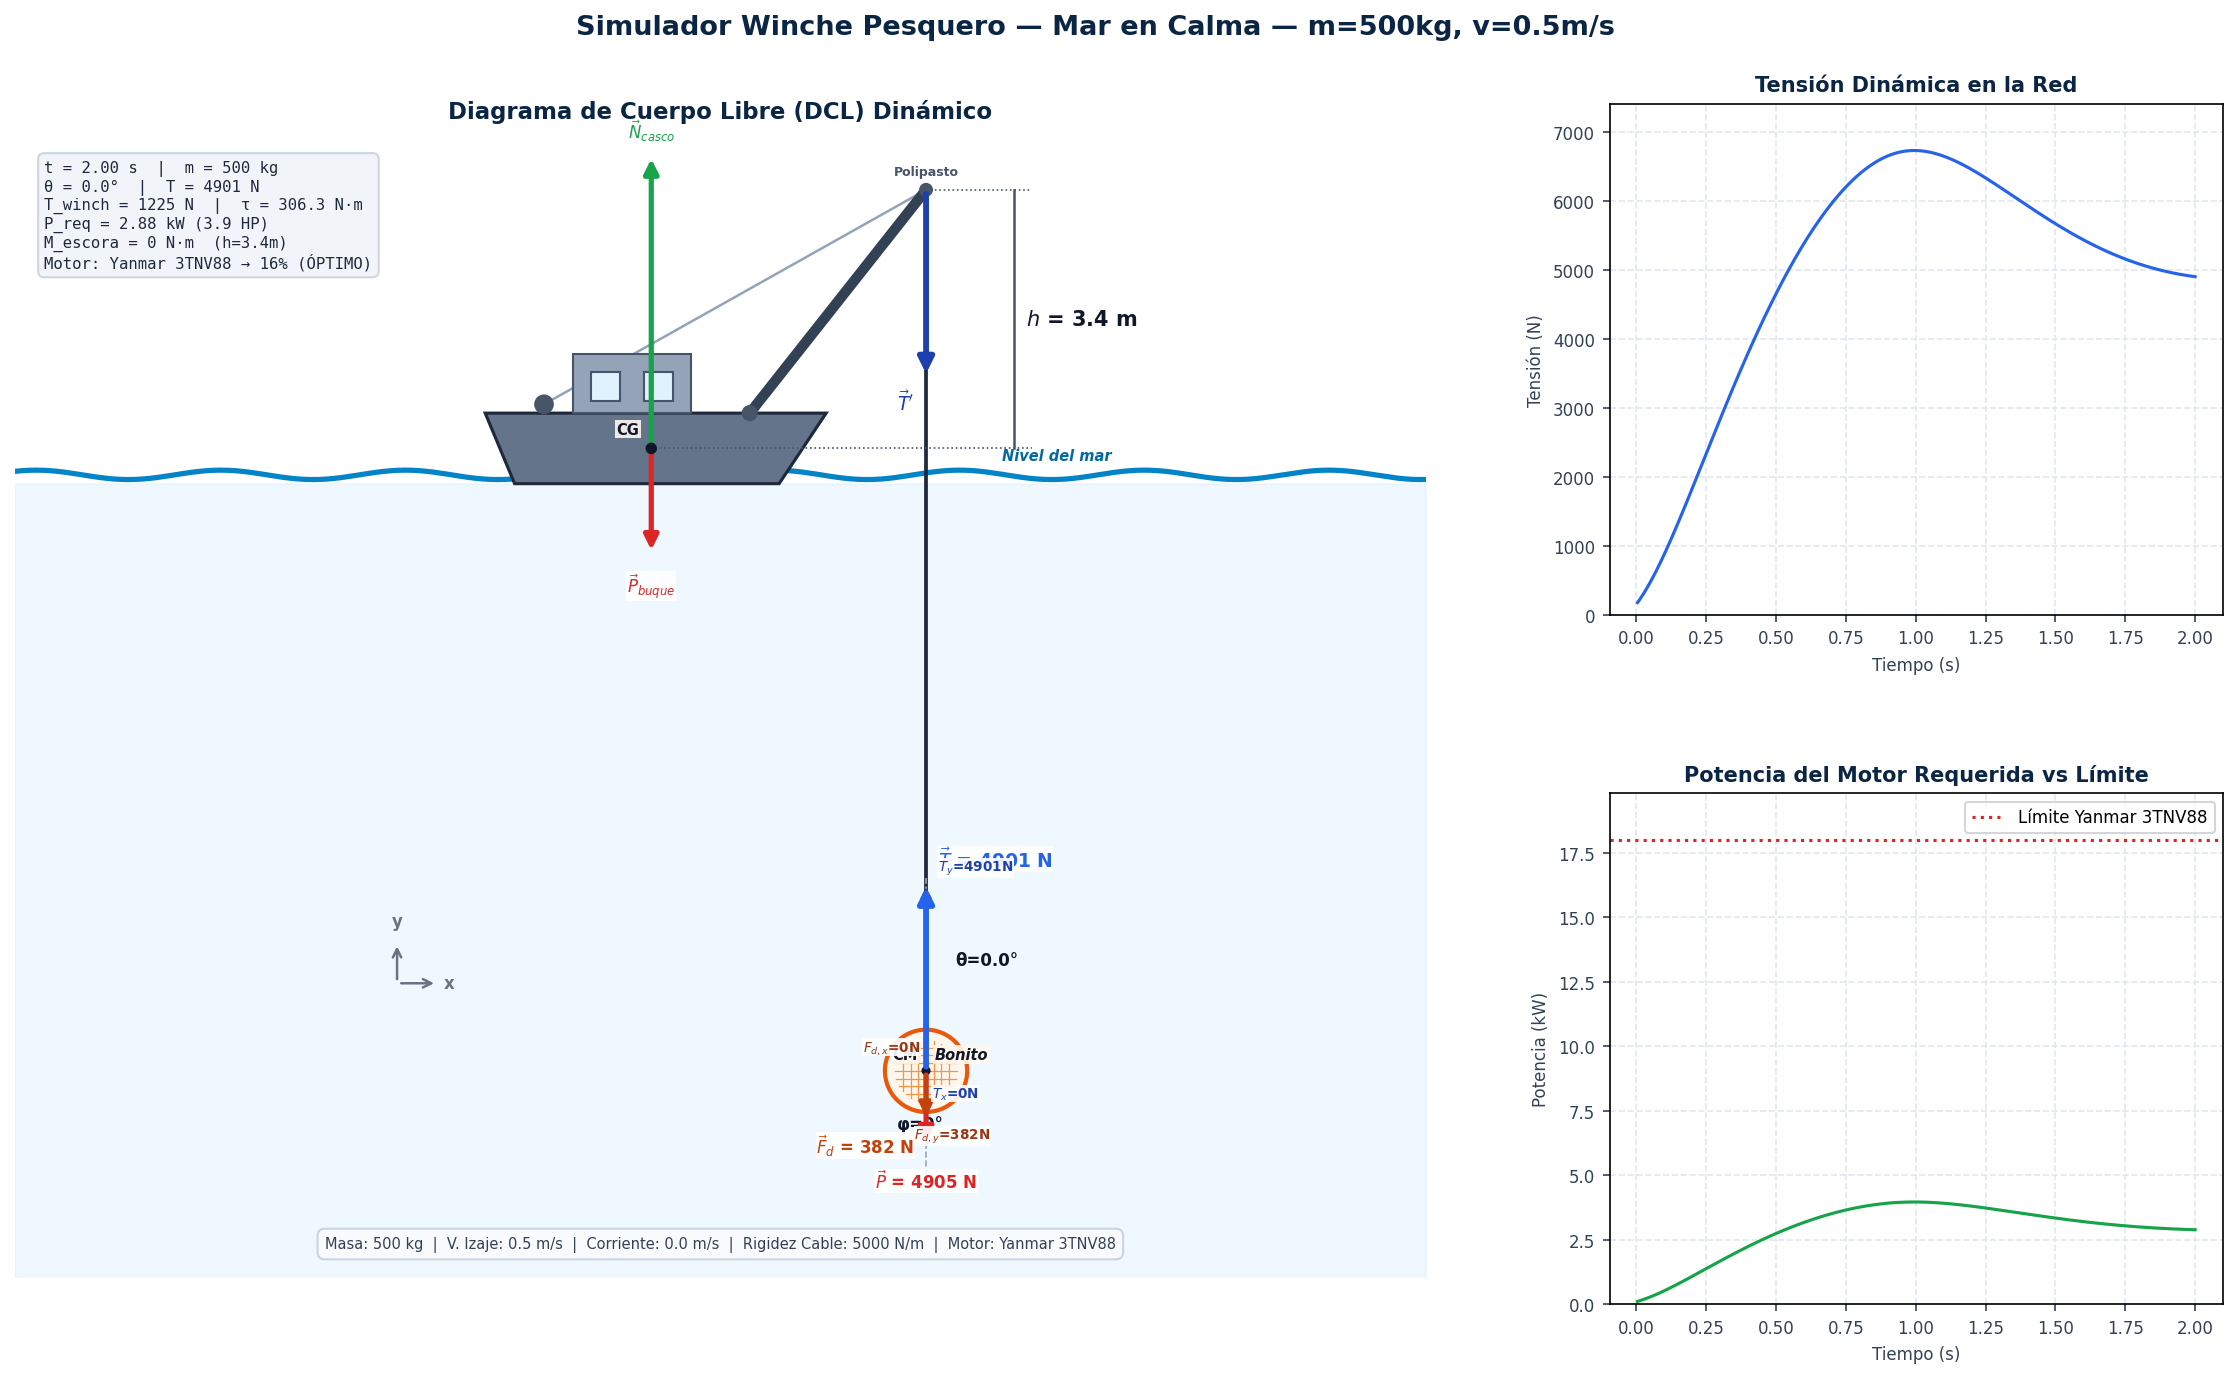
\includegraphics[width=0.85\textwidth]{simulacion/prueba1_mar_calma.png}
    \caption{Simulación en mar en calma: el cable permanece vertical y la telemetría coincide con el equilibrio estático de fuerzas.}
    \label{fig:prueba1}
\end{figure}

\subsubsection{Prueba 2: Izaje bajo Efecto de Corriente Marina Transversal}
Corresponde a las condiciones de diseño críticas del Escenario 2 ($m = \SI{500}{kg}$, $v_{\text{izaje}} = \SI{0.5}{m/s}$, $v_{\text{corriente}} = \SI{1,5}{m/s}$). La corriente transversal desplaza lateralmente la red cargada.
\begin{itemize}
    \item \textbf{Tensión total en el cable ($T$):} \SI{6028}{N}.
    \item \textbf{Ángulo del cable ($\theta$):} $21,2^\circ$ respecto a la vertical.
    \item \textbf{Potencia requerida por el motor ($P_{\text{req}}$):} \SI{3,55}{kW}.
    \item \textbf{Momento de escora ($M_e$):} \SI{7398}{N.m} (a una altura del boom $h = \SI{3,4}{m}$).
    \item \textbf{Estado del motor (Yanmar 3TNV88):} Óptimo (carga moderada, $\approx 20\%$).
\end{itemize}
La fuerza horizontal de la corriente y la inclinación del cable incrementan notablemente la tensión total y provocan un momento de escora sobre el buque que debe ser monitoreado para la estabilidad naval.

\begin{figure}[H]
    \centering
    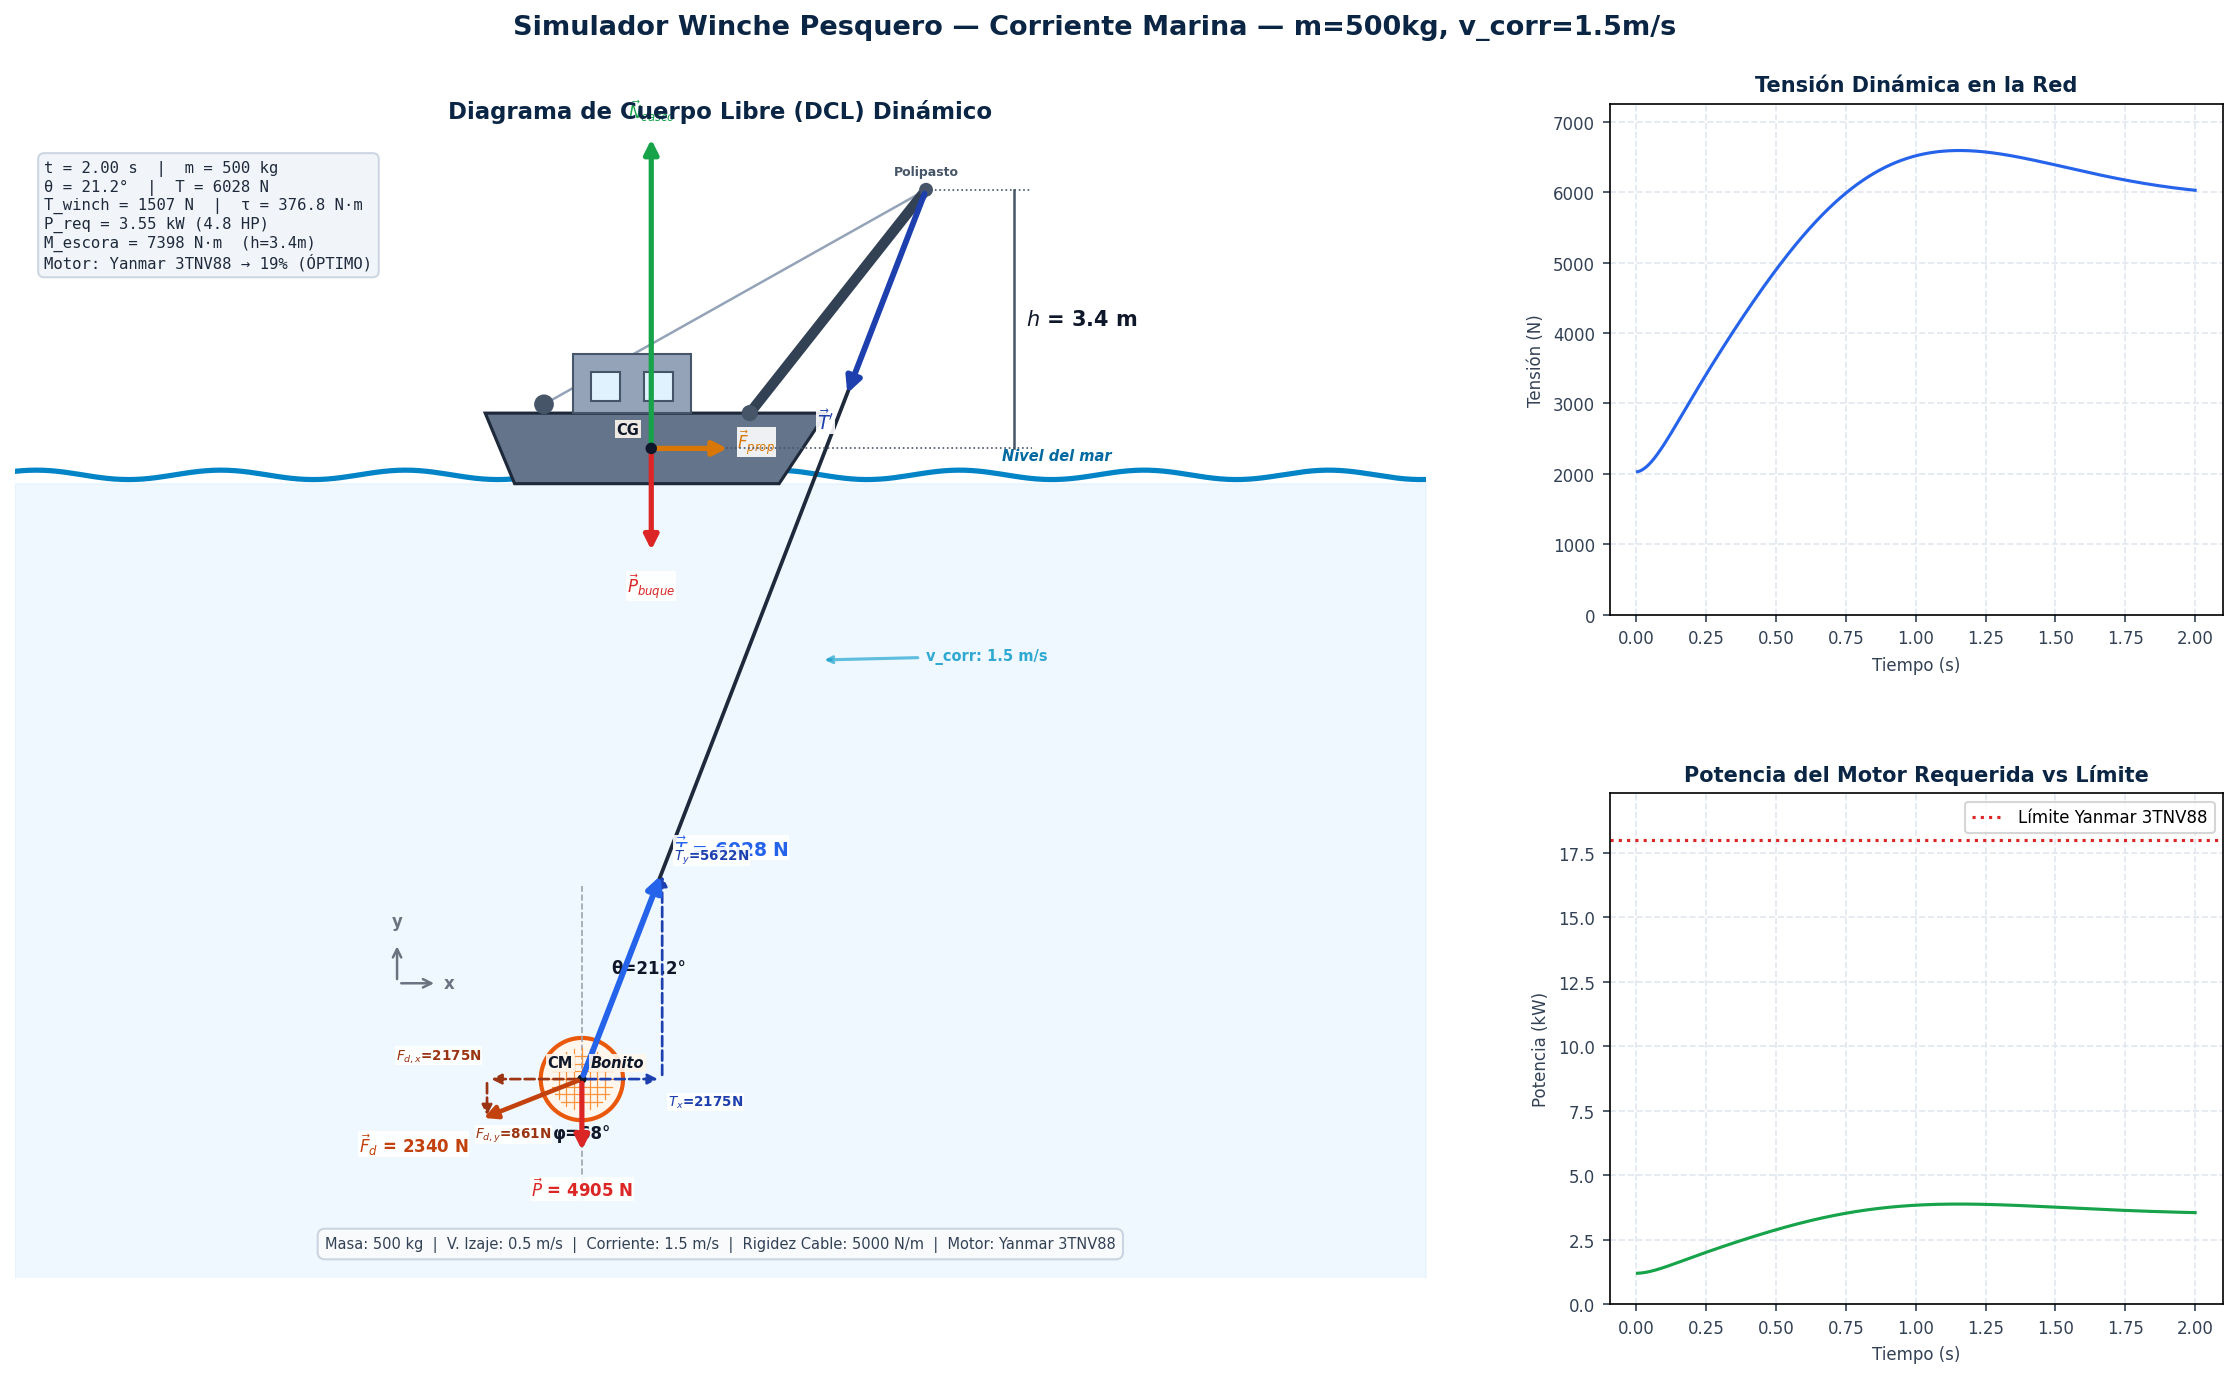
\includegraphics[width=0.85\textwidth]{simulacion/prueba2_corriente_1_5.png}
    \caption{Simulación con corriente marina transversal de \SI{1,5}{m/s}: se aprecia la inclinación del cable ($\theta \approx 21,2^\circ$) y el correspondiente momento de escora.}
    \label{fig:prueba2}
\end{figure}

\subsubsection{Prueba 3: Operación a Carga Máxima}
Se evalúa un escenario extremo de izaje de captura masiva de bonito ($m = \SI{1500}{kg}$) manteniendo la velocidad de izaje en \SI{0,5}{m/s} y bajo la corriente transversal estándar de \SI{1,5}{m/s}.
\begin{itemize}
    \item \textbf{Tensión total en el cable ($T$):} \SI{17242}{N}.
    \item \textbf{Ángulo del cable ($\theta$):} $14,1^\circ$.
    \item \textbf{Potencia requerida por el motor ($P_{\text{req}}$):} \SI{10,14}{kW}.
    \item \textbf{Momento de escora ($M_e$):} \SI{14310}{N.m}.
    \item \textbf{Estado del motor (Yanmar 3TNV88):} Óptimo (carga de trabajo pesada, $\approx 56\%$).
\end{itemize}
Aunque la masa de bonito se triplica, el ángulo $\theta$ disminuye a $14,1^\circ$ debido al mayor peso en la vertical ($P = \SI{14715}{N}$) en relación con el arrastre hidrodinámico. El motor Yanmar 3TNV88 demuestra su idoneidad al soportar holgadamente esta maniobra crítica de izaje.

\begin{figure}[H]
    \centering
    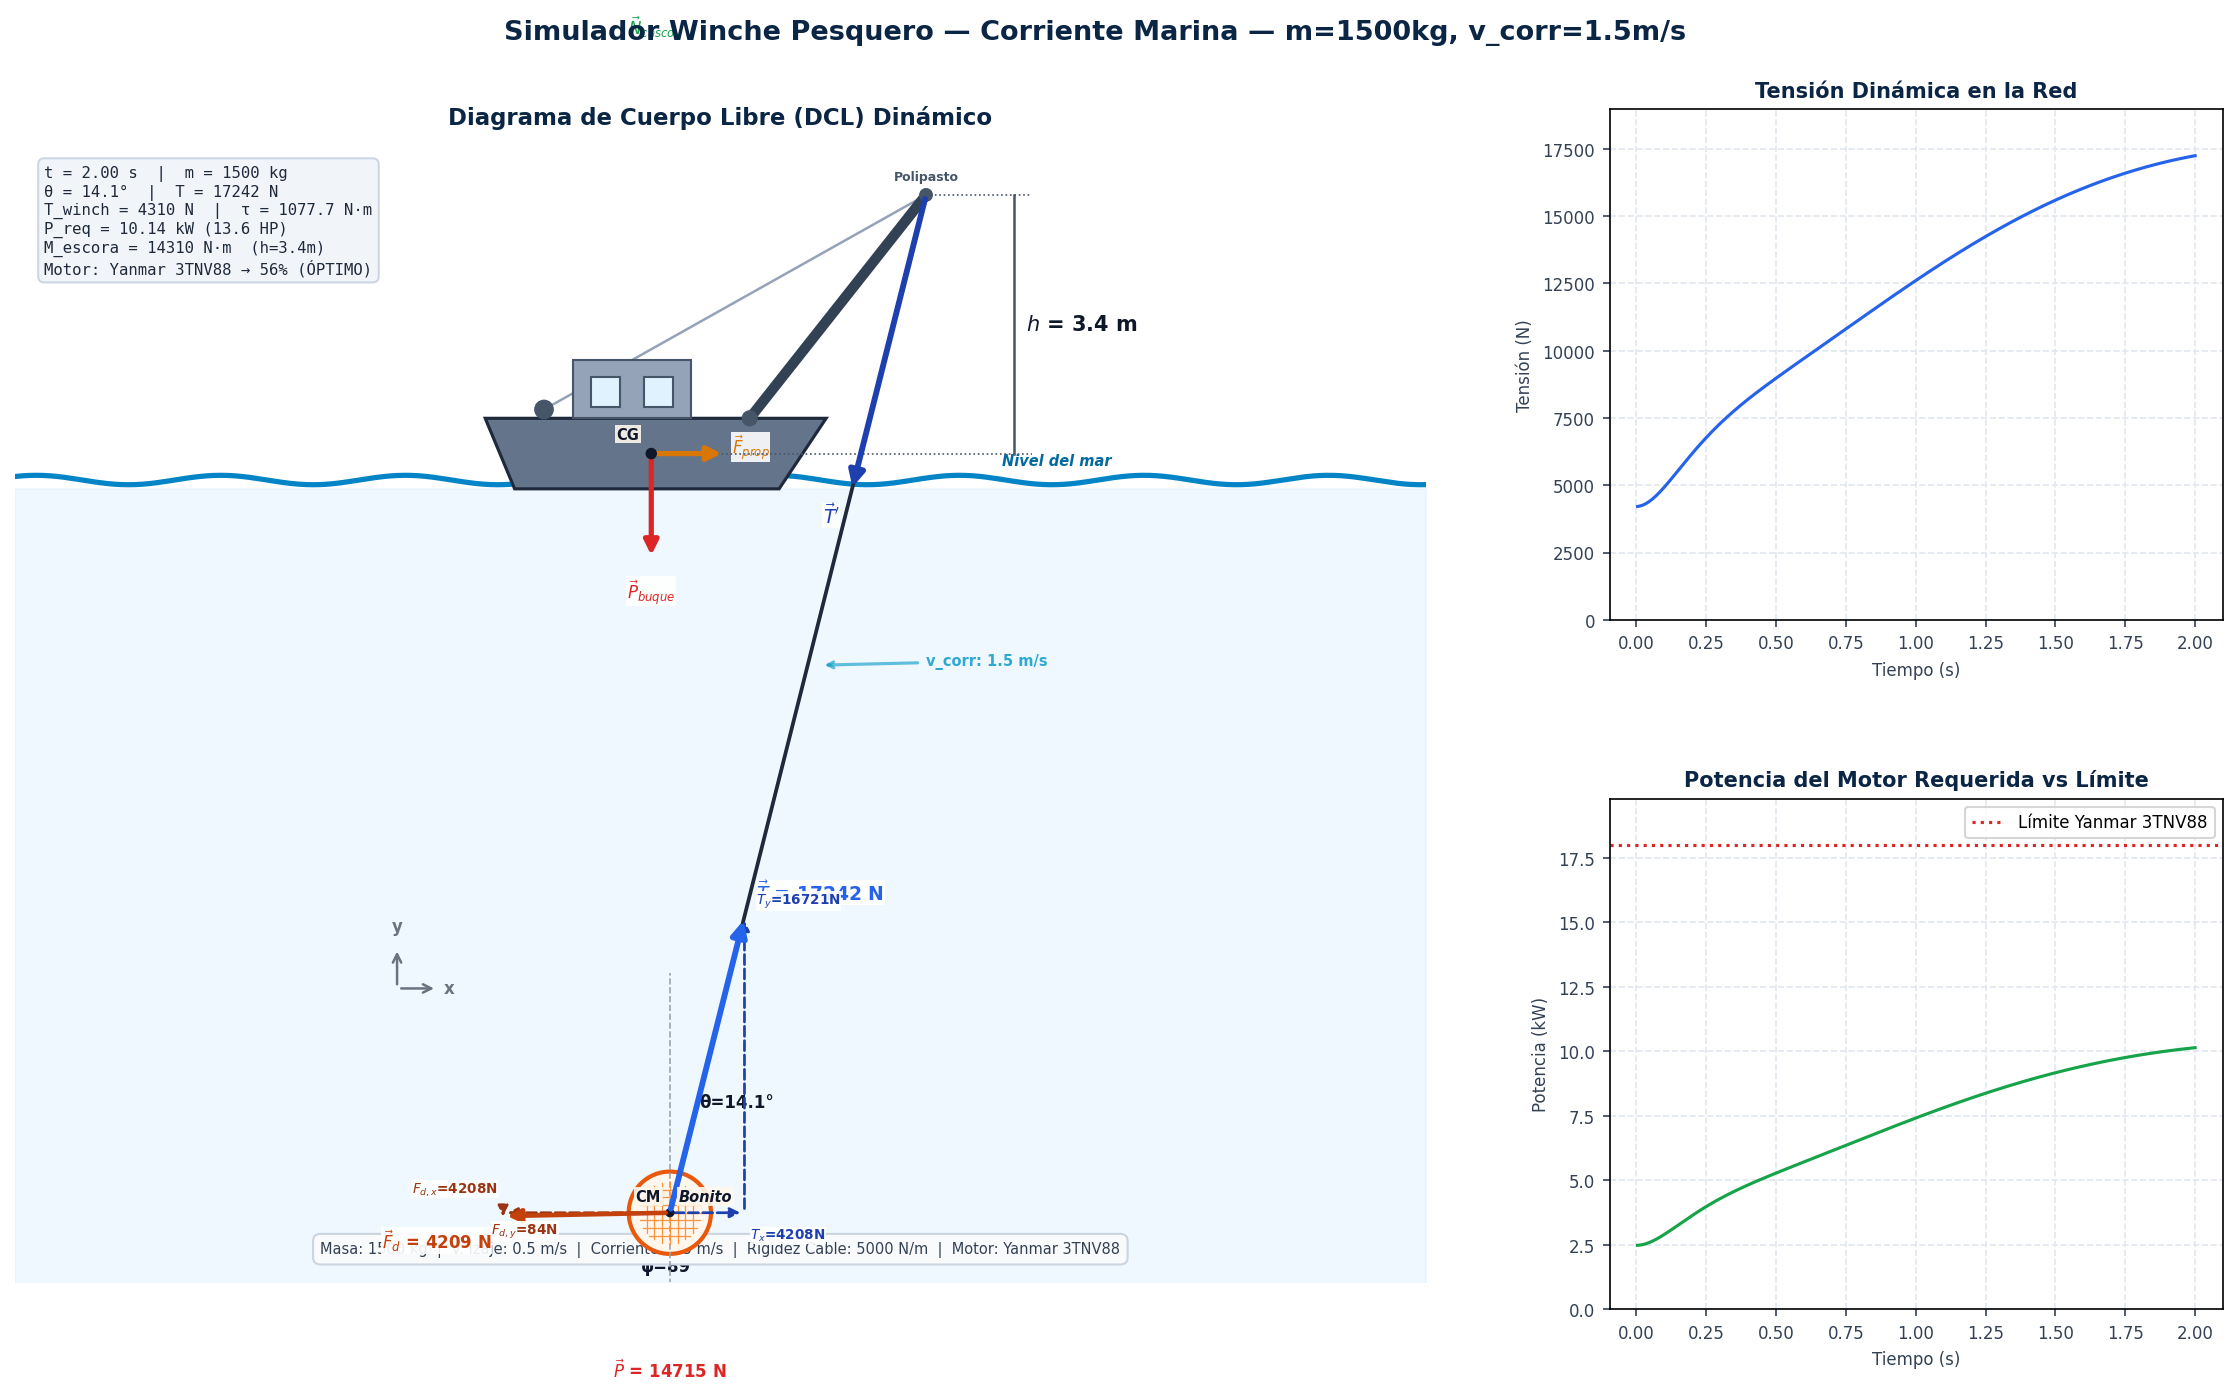
\includegraphics[width=0.85\textwidth]{simulacion/prueba3_carga_maxima.png}
    \caption{Simulación a carga máxima ($m = \SI{1500}{kg}$): el motor Yanmar 3TNV88 opera de forma segura al $56\%$ de su potencia nominal.}
    \label{fig:prueba3}
\end{figure}

\subsubsection{Prueba 4: Alta Velocidad de Izaje}
Se analiza un izaje rápido de la captura ($v_{\text{izaje}} = \SI{2,0}{m/s}$) bajo condiciones de carga estándar ($m = \SI{500}{kg}$) y corriente transversal de \SI{1,5}{m/s}.
\begin{itemize}
    \item \textbf{Tensión total en el cable ($T$):} \SI{9943}{N}.
    \item \textbf{Ángulo del cable ($\theta$):} $19,7^\circ$.
    \item \textbf{Potencia requerida por el motor ($P_{\text{req}}$):} \SI{23,40}{kW}.
    \item \textbf{Momento de escora ($M_e$):} \SI{11411}{N.m}.
    \item \textbf{Estado del motor (Yanmar 3TNV88):} \textbf{¡SOBRECARGA!} ($\approx 130\%$).
\end{itemize}
Al elevar a alta velocidad, la potencia requerida se dispara debido al trabajo mecánico rápido, superando la potencia límite de \SI{18,0}{kW} del Yanmar 3TNV88. Esto genera una alarma visual en el simulador y evidencia la necesidad de limitar la velocidad del winche durante el virado.

\begin{figure}[H]
    \centering
    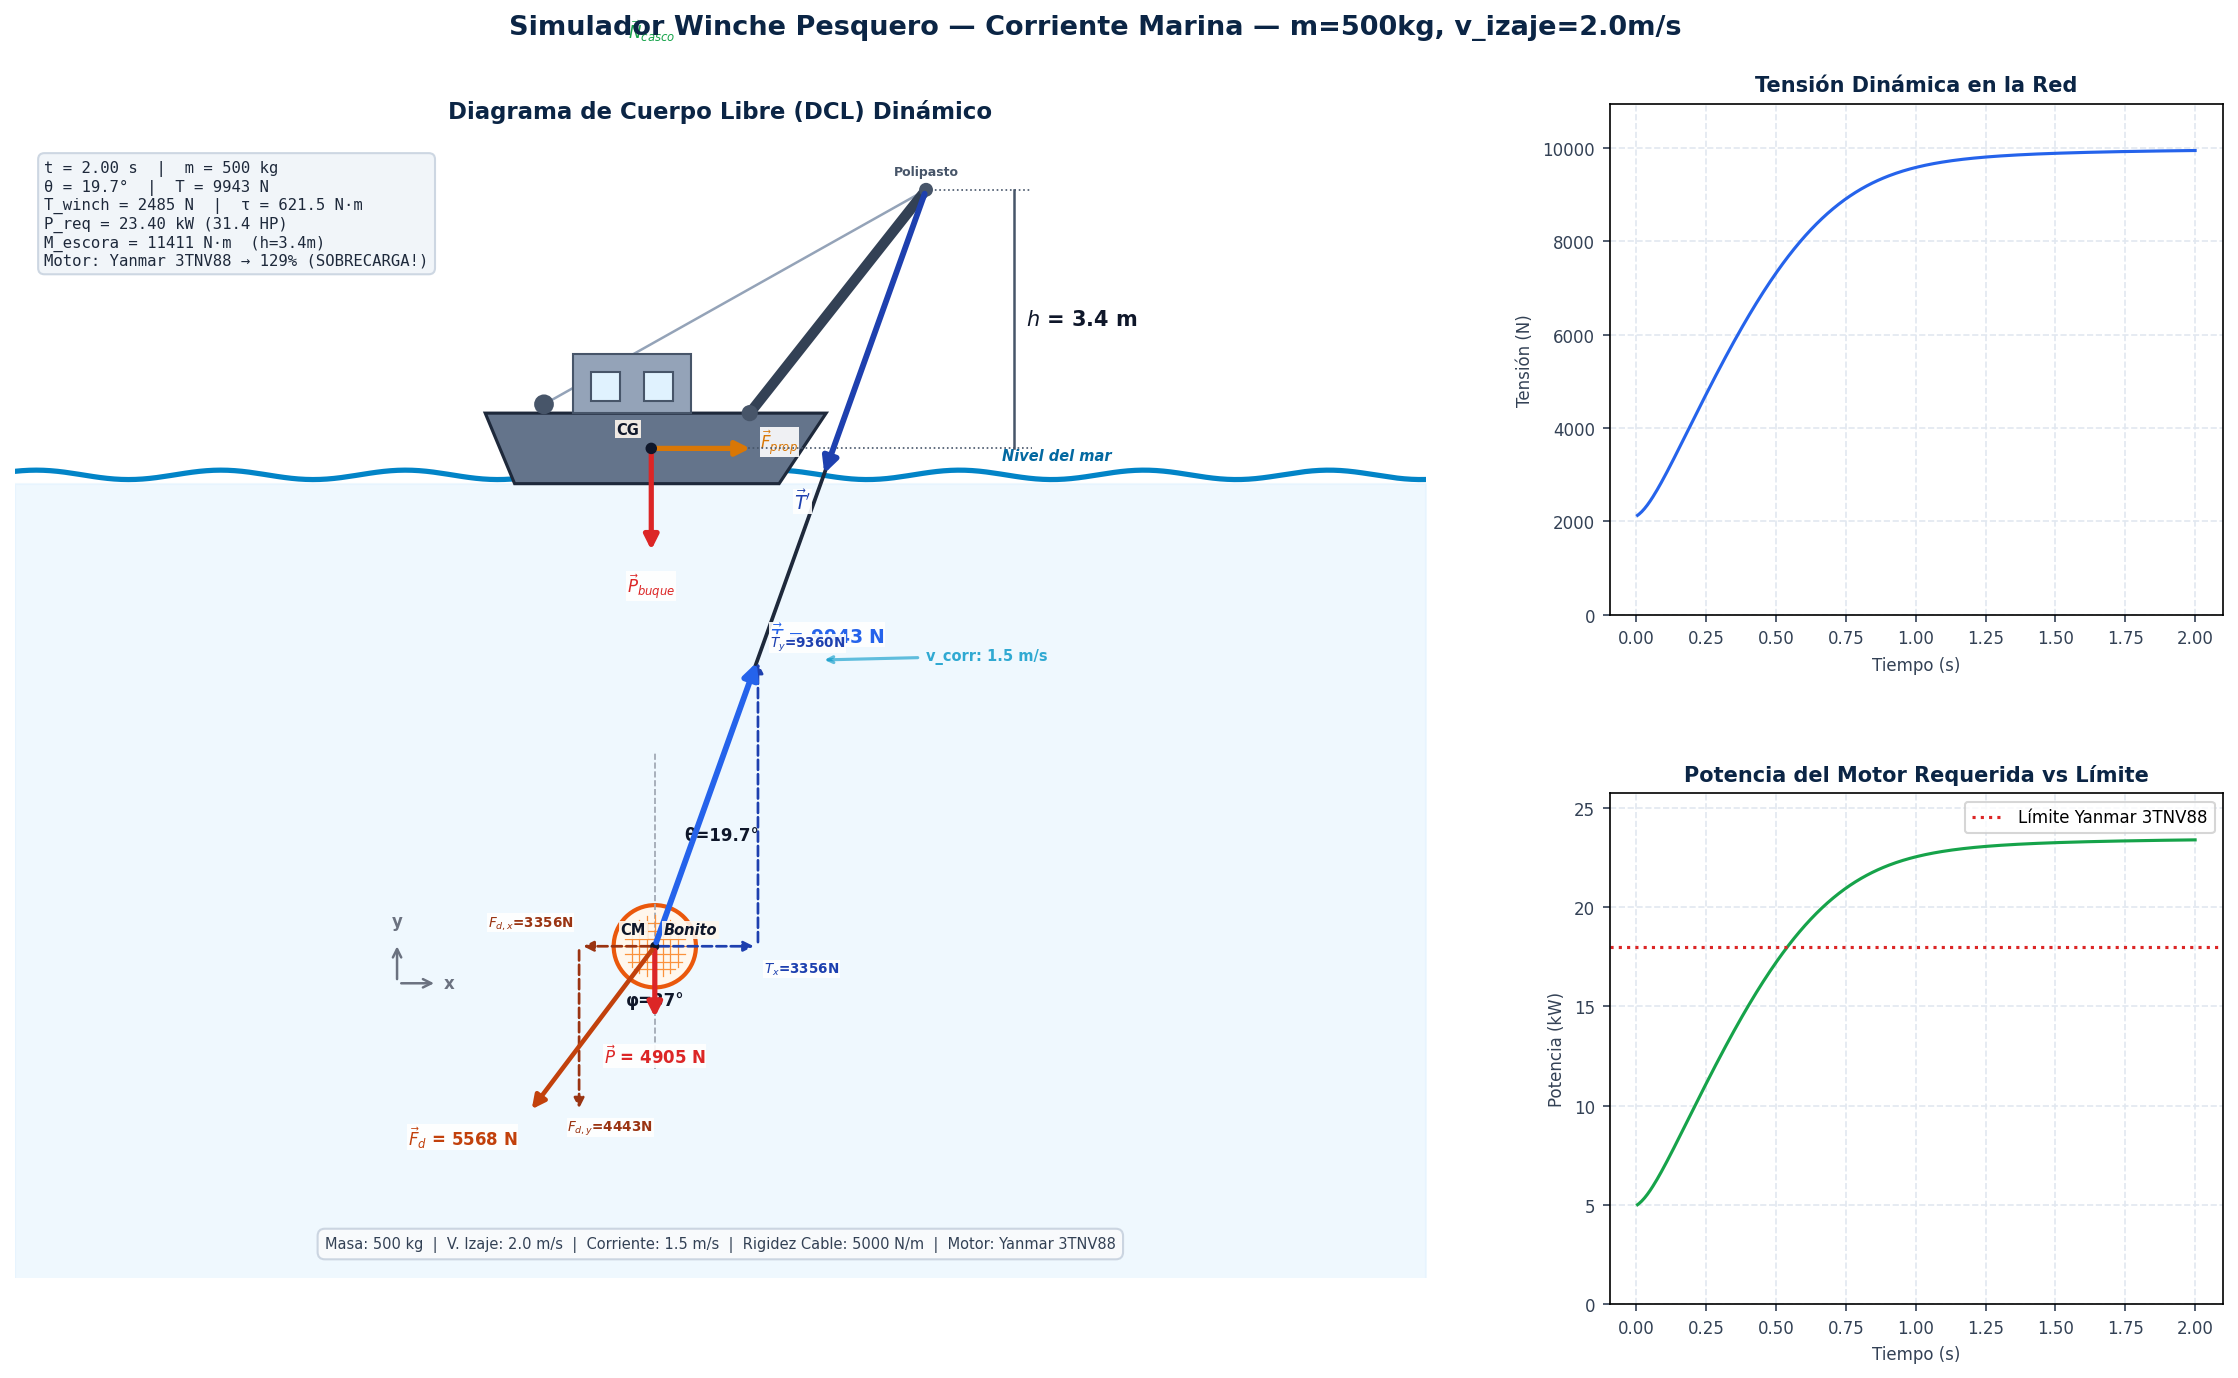
\includegraphics[width=0.85\textwidth]{simulacion/prueba4_alta_velocidad.png}
    \caption{Simulación a alta velocidad de izaje: el panel de control y las gráficas advierten sobrecarga por superar la capacidad nominal del motor.}
    \label{fig:prueba4}
\end{figure}

\subsubsection{Prueba 5: Selección de Motor Inadecuado bajo Condiciones de Tempestad}
Se simula el izaje con el motor más pequeño de la comparativa (\textit{Chongqing Mini}, con límite de \SI{12,0}{kW}) ante una biomasa de \SI{1000}{kg}, velocidad del winche de \SI{1,0}{m/s} y corriente marina severa de \SI{2,0}{m/s}.
\begin{itemize}
    \item \textbf{Tensión total en el cable ($T$):} \SI{14622}{N}.
    \item \textbf{Ángulo del cable ($\theta$):} $25,6^\circ$.
    \item \textbf{Potencia requerida por el motor ($P_{\text{req}}$):} \SI{17,20}{kW}.
    \item \textbf{Momento de escora ($M_e$):} \SI{21465}{N.m}.
    \item \textbf{Estado del motor (Chongqing Mini):} \textbf{¡SOBRECARGA CRÍTICA!} ($\approx 143\%$).
\end{itemize}
El motor Chongqing Mini queda completamente sobrepasado por la combinación de velocidad, corriente y carga, lo que resultaría en una falla de velocidad o detención térmica en una maniobra real. Asimismo, el momento de escora es muy elevado (\SI{21465}{N.m}), comprometiendo la estabilidad lateral.

\begin{figure}[H]
    \centering
    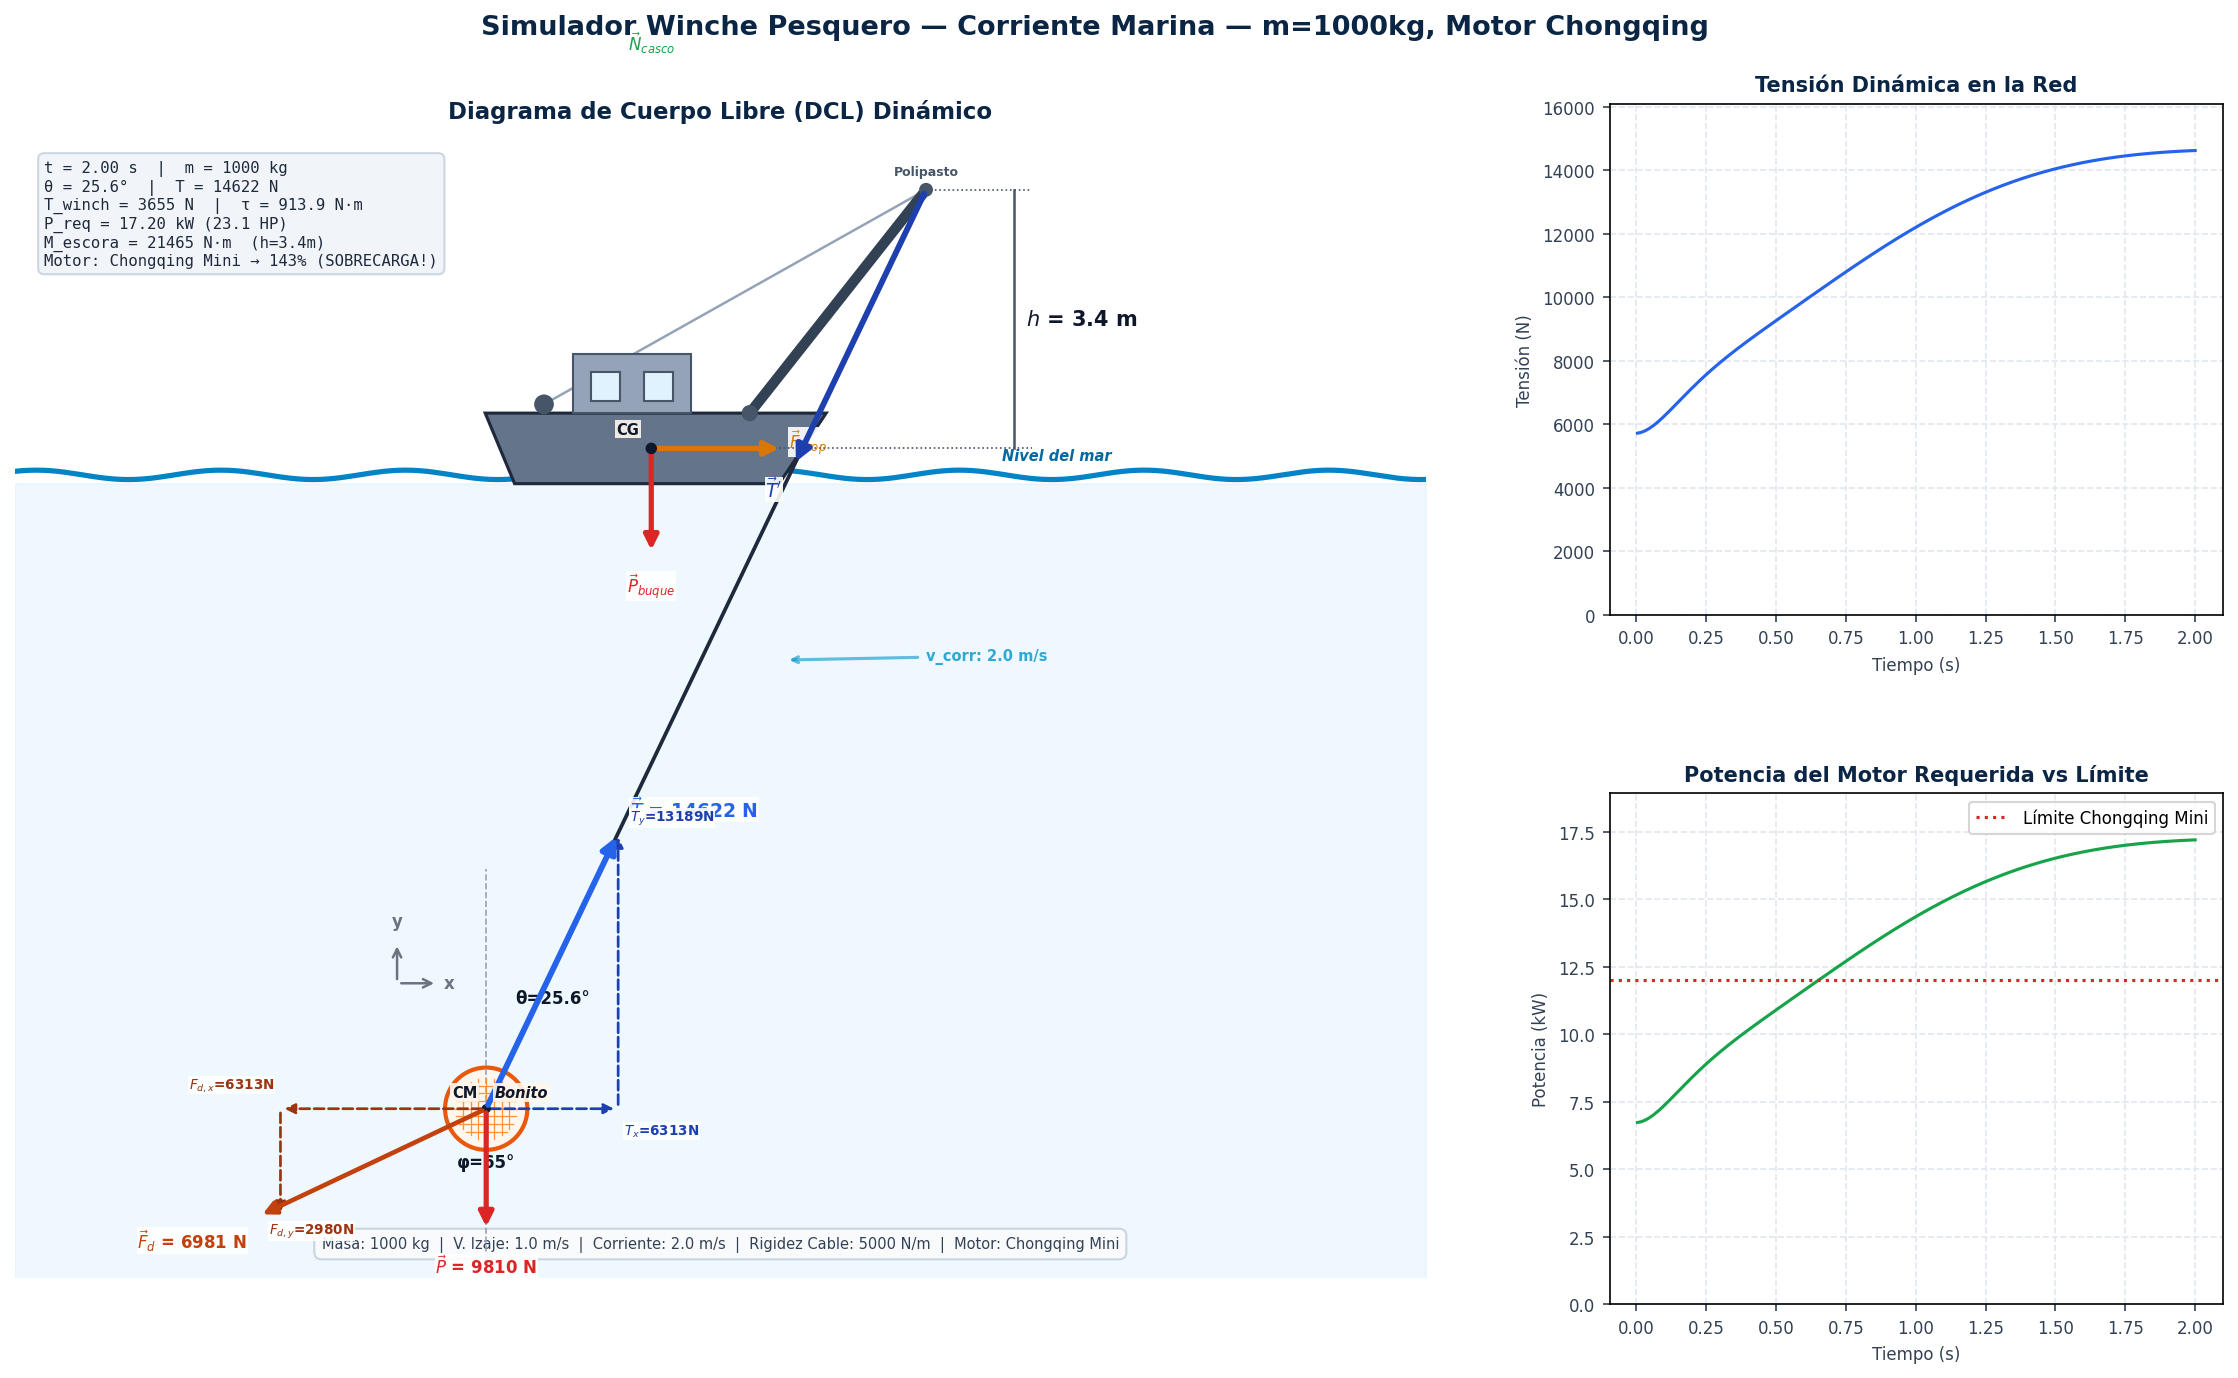
\includegraphics[width=0.85\textwidth]{simulacion/prueba5_motor_sobrecarga.png}
    \caption{Simulación de motor inadecuado: la combinación de variables dinámicas sobrepasa en un $143\%$ la capacidad de diseño del motor Chongqing Mini.}
    \label{fig:prueba5}
\end{figure}

\section{Justificación e Importancia en nuestra Formación Profesional}
El diseño de maquinaria de cubierta y la planificación de las operaciones de extracción pesquera no pueden basarse en aproximaciones empíricas. Este análisis demuestra que el conocimiento de la Física I (cinemática lineal, estática, dinámica de Newton, leyes de conservación de energía y mecánica de fluidos) es el núcleo del diseño y la seguridad operativa de la flota pesquera. 

Comprender la dinámica de fuerzas inerciales y de arrastre capacita al futuro ingeniero para seleccionar componentes mecánicos y motores bajo criterios científicos rigurosos, evitando pérdidas materiales o riesgos humanos. Asimismo, vincula la física pura con tecnologías de simulación y diseño tridimensional asistido por computadora (CAD), esenciales para la modernización y automatización de los barcos pesqueros en la era industrial actual.


\section{Referencias}
\begin{itemize}
    \item FAO. (2022). \textit{El estado mundial de la pesca y la acuicultura 2022. Hacia la transformación azul}. Organización de las Naciones Unidas para la Alimentación y la Agricultura. \url{https://doi.org/10.4060/cc0461es}
    \item García, M., López, J., \& Rodríguez, C. (2019). \textit{Mecánica aplicada en la ingeniería naval y pesquera} (2.ª ed.). Ediciones Académicas.
    \item Hewitt, P. G. (2016). \textit{Física conceptual} (12.ª ed.). Pearson Educación.
    \item Pérez, A., \& Martínez, L. (2021). Automatización y sensores en la maquinaria de cubierta para buques pesqueros. \textit{Revista de Ingeniería Marítima}, 14(2), 45-60.
    \item Serway, R. A., \& Jewett, J. W. (2018). \textit{Física para ciencias e ingeniería} (10.ª ed., Vol. 1). Cengage Learning.
    \item Young, H. D., \& Freedman, R. A. (2018). \textit{Física universitaria con física moderna} (14.ª ed., Vol. 1). Pearson Educación.
\end{itemize}

\end{document}
